\documentclass[11pt,a4paper]{article}
% Needed for arxiv
\usepackage[hyperref]{style/acl2021}
\usepackage{times}
\usepackage{latexsym}
\usepackage{url}
\usepackage{booktabs}
\usepackage{tikz}
\usepackage[utf8]{inputenc}
\usepackage[T1]{fontenc}
\usepackage{anyfontsize}
\usepackage{caption}
\usepackage{subcaption}
\usepackage{xstring}
\usepackage{todonotes}
\usepackage{csquotes}
\usepackage{pifont}% http://ctan.org/pkg/pifont
\usepackage{mathtools}
\usepackage{xcolor}
\usepackage{enumitem}
\newcommand{\hl}[1]{\colorbox{yellow}{#1}}
\newcommand{\hz}{\vphantom{\parbox[c]{0.1cm}{\rule{0.1cm}{0.4cm}}}}

% Anonymity macros
\aclfinalcopy % Uncomment this line for the final submission
\def\aclpaperid{896} %  Enter the acl Paper ID here
\newcommand{\projecturl}{\href{https://irt.pedro.ai}{irt.pedro.ai}}
%%%%%%%%%%%%%%%%%%%%%%%% Author added %%%%%%%%%%%%%%%%%%%%%%%%

\newif\ifcomment
%\commenttrue
\commentfalse

% Preamble file contains handy macros and most packages you might want to use.
% At the start are packages that conflict with various styles.  Don't add them
% in!  Just put it in your main TeX file instead.

% Do not put either of these (subfigure or subfloat) into the preamble
% - they clash.  Use them in the final LaTeX document
% \usepackage{subfigure}
% \suepackage{subfloat}

% Do not use times in the preamble!  It just causes problems with some
% publication chairs (e.g., ICML 2013).  If you want it, put it in your own
% document.
% \usepackage{times}


% Breaks ACM-SIG style
% \usepackage{titlesec}
% \usepackage{amsthm}
% \usepackage{nomencl}

% comment out the following line, as it conflicts with aistats2012.sty
%\usepackage{caption}


% Below should be safe
\usepackage{framed}
\usepackage{mdwlist}
\usepackage{latexsym}
\usepackage{xcolor}
\usepackage{nicefrac}
\usepackage{booktabs}
\usepackage{amsfonts}
\usepackage[T1]{fontenc}
\usepackage{bold-extra}
\usepackage{amsmath}
\usepackage{dsfont}
\usepackage{amssymb}
\usepackage{bm}
\usepackage{graphicx}
\usepackage{mathtools}
\usepackage{microtype}
\usepackage{multirow}
\usepackage{multicol}
%\usepackage{url}
\usepackage{latexsym,comment}

\newcommand{\breakalign}{\right. \nonumber \\ & \left. \hspace{2cm}}



\newcommand{\feat}[1]{{\small \texttt{#1}}}
\newcommand{\act}[1]{{\small \texttt{#1}}}
\newcommand{\ngram}[0]{$n$-gram}
\newcommand{\gem}[1]{\mbox{\textsc{gem}}}
\newcommand{\abr}[1]{\textsc{#1}}
\newcommand{\camelabr}[2]{{\small #1}{\textsc{#2}}}
\newcommand{\abrcamel}[2]{{\textsc #1}{\small{#2}}}
\newcommand{\grammar}[1]{{\color{red} #1}}
\newcommand{\explain}[2]{\underbrace{#2}_{\mbox{\footnotesize{#1}}}}
\newcommand{\dir}[1]{\mbox{Dir}(#1)}
\newcommand{\bet}[1]{\mbox{Beta}(#1)}
\newcommand{\py}[1]{\mbox{\textsc{py}}(#1)}
\newcommand{\td}[2]{\mbox{\textsc{TreeDist}}_{#1} \left( #2 \right)}
\newcommand{\yield}[1]{\mbox{\textsc{Yield}} \left( #1 \right)}
\newcommand{\mult}[1]{\mbox{Mult}( #1)}
\newcommand{\wn}{\textsc{WordNet}}
\newcommand{\twentynews}{\textsc{20news}}
\newcommand{\g}{\, | \,}
\newcommand{\Gam}[1]{\Gamma \left( \textstyle #1 \right)}
\newcommand{\LG}[1]{\log \Gamma \left( \textstyle #1 \right)}
\newcommand{\Pois}[1]{\mbox{Poisson}(#1)}
\newcommand{\pcfg}[3]{#1_{#2 \rightarrow #3}}
\newcommand{\grule}[2]{#1 \rightarrow #2}
\newcommand{\kl}[2]{D_{\mbox{\textsc{KL}}} \left( #1 \,||\, #2 \right)}

\newcommand{\digambig}[1]{\Psi \left( #1 \right) }
\newcommand{\digam}[1]{\Psi \left( \textstyle #1 \right) }
\newcommand{\ddigam}[1]{\Psi' \left( \textstyle #1 \right) }

\DeclareMathOperator*{\argmax}{arg\,max}
\DeclareMathOperator*{\argmin}{arg\,min}
\newcommand{\bmat}[1]{\text{\textbf{#1}}}
\newcommand{\bvec}[1]{\boldsymbol{#1}}

%\newcommand{\email}[1]{ {\small \href{mailto://#1}{\texttt{#1} }  }}
\newcommand{\emaillink}[1]{ {\small \href{mailto://#1}{\texttt{#1}}}}
\newcommand{\smallemaillink}[2]{ {\small \href{mailto://#2}{\texttt{#1}}}}

% JBG: Consider renaming from \ch to \zh because of conflict when adding Cyrillic
\newcommand{\ch}[1]{\begin{CJK*}{UTF8}{gbsn}#1\end{CJK*}}

\newcommand{\e}[2]{\mathbb{E}_{#1}\left[ #2 \right] }
\newcommand{\h}[2]{\mathbb{H}_{#1}\left[ #2 \right] }
\newcommand{\ind}[1]{\mathds{1}\left[ #1 \right] }
\newcommand{\ex}[1]{\mbox{exp}\left\{ #1\right\} }
\newcommand{\D}[2]{\frac{\partial #1}{\partial #2}}
\newcommand{\elbo}{\mathcal{L}}

\newcommand{\hidetext}[1]{}
\newcommand{\ignore}[1]{}

\newcommand{\todo}[1]{\textcolor{red}{{\bf TODO: #1}}}

\ifcomment
    \newcommand{\pinaforecomment}[3]{\colorbox{#1}{\parbox{.8\linewidth}{#2: #3}}}
\else
    \newcommand{\pinaforecomment}[3]{}
\fi

\newcommand{\prcomment}[1]{\pinaforecomment{lightblue}{Pedro}{#1}}
\newcommand{\paulcomment}[1]{\pinaforecomment{orange}{Paul}{#1}}
\newcommand{\stephencomment}[1]{\pinaforecomment{yellow}{Stephen}{#1}}
\newcommand{\shane}[1]{\pinaforecomment{blue}{Shane}{#1}}
\newcommand{\anyone}[1]{\pinaforecomment{yellow}{Anyone}{#1}}

\newcommand{\smalltt}[1]{ {\tt \small #1 }}
\newcommand{\smallurl}[1]{ \begin{tiny}\url{#1}\end{tiny}}
%\newcommand{\smallurl}[1]{ \begin{tiny} HIDDEN \end{tiny}}
\newenvironment{compactenum}{ \begin{enumerate*} \small }{ \end{enumerate*} }

\definecolor{lightblue}{HTML}{3cc7ea}
\definecolor{CUgold}{HTML}{CFB87C}
\definecolor{grey}{rgb}{0.95,0.95,0.95}
\definecolor{ceil}{rgb}{0.57, 0.63, 0.81}
\definecolor{vyellow}{HTML}{d1c73b}
\newcommand*{\TakeFourierOrnament}[1]{{%
            \fontencoding{U}\fontfamily{futs}\selectfont\char#1}}
\newcommand*{\danger}{\TakeFourierOrnament{66}}
\newcommand\cmark {\textcolor{green}{\ding{52}}}
\newcommand\xmark {\textcolor{red}{\ding{55}}}
\newcommand\dmark {\textcolor{vyellow}{\danger}}


% Datasets / Models

\newcommand{\qb}[0]{Quizbowl}
\newcommand{\triviaqa}{\camelabr{Trivia}{qa}}
\newcommand{\qblink}{\abrcamel{qb}{Link}}
\newcommand{\qanta}{\textsc{qanta}}
\newcommand{\muse}{\textsc{muse}}
\newcommand{\squad}{\textsc{sq}{\small u}\textsc{ad}}
\newcommand{\elmo}{\textsc{elm}{\small o}}
\newcommand{\coqa}{\textsc{c}{\small o}\textsc{q}{\small a}}
\newcommand{\quac}{\textsc{q}{\small u}\textsc{ac}}
\newcommand{\glove}{\abr{gl}{\small o}\abr{ve}}
\newcommand{\opendialkg}{\abr{o}{\small pen}\abr{d}{\small ial}\abr{kg}}
\newcommand{\mrr}{\abr{mrr}}
\newcommand{\fone}{\abr{f}$_1$}
\newcommand{\tfidf}{\abr{tf-idf}}
\newcommand{\hre}{\abr{hre}}
\newcommand{\parlai}{\abr{p}{\small arl}\abr{ai}}
\newcommand{\wow}{\abr{w}{\small o}\abr{w}}
\newcommand{\bilstm}{\abr{b}{\small i}\abr{lstm}}
\newcommand{\woz}{\abr{w}{\small o}\abr{z}}
\newcommand{\allennlp}{\abr{A}{\small llen}\abr{nlp}}
\newcommand{\saac}{\abr{s}{\small aa}\abr{c}}
\newcommand{\cast}{\abr{ca}{\small s}\abr{t}}
\newcommand{\charm}{\abr{charm}}
\newcommand{\emailcustom}[2]{ {\small \href{mailto://#1}{\texttt{#2}}}}
\newcommand{\irt}{\abr{irt}}
\newcommand{\iemph}[1]{\textit{#1}}
\newcommand{\trec}{\abr{trec}}
\newcommand{\ir}{\abr{ir}}
\newcommand{\itm}{item}
\newcommand{\itms}{items}
\newcommand{\Itms}{Items}
\newcommand{\Itm}{Item}
\newcommand{\name}{\abr{dad}}
\newcommand{\subj}{subject}
\newcommand{\subjs}{subjects}
\newcommand{\Subj}{Subject}
\newcommand{\resp}{response}
\newcommand{\resps}{responses}
\newcommand{\Resp}{Response}
\newcommand{\nsquadsubj}{0}
\newcommand{\discability}{discriminability}
\newcommand{\diff}{difficulty}
\newcommand{\Diff}{Difficulty}
\newcommand{\smart}{Ken}
\newcommand{\dumb}{Burt}

\newcommand{\Discability}{Discriminability}
\newcommand{\answer}[1]{{\color{red}#1}}
\newcommand{\pl}[1]{%
\IfStrEqCase{#1}{{1}{\abr{irt}-base}
    {2}{\abr{irt}-disc}
    {3}{\abr{irt}-feas}
    {m}{\abr{irt}-vec}
    {t}{\abr{irt}-tm}    
  }
}
\newcommand{\terp}{
\includegraphics[scale=0.02]{2021_acl_leaderboard/figures/redshell}}
\newcommand{\sterp}{\textsuperscript{
\includegraphics[scale=0.02]{2021_acl_leaderboard/figures/redshell}}}
% In order, prefer figures from
% Hand made: figures
% Auto generated and committed: commit_auto_fig
% Auto generated: auto_fig
% The concept is to promote auto_fig figures to commit_auto_fig
% This is particularly important so that figures can appear in paper correctly
% even if the builder of the paper doesn't have the data
\graphicspath{{2021_acl_leaderboard/figures/}{2021_acl_leaderboard/commit_auto_figs/}{2021_acl_leaderboard/auto_fig/}}
%%%%%%%%%%%%%%%%%%%%%%%%%%%%%%%%%%%%%%%%%%%%%%%%%%%%%%%%%%%%%%

\title{Evaluation Examples Are Not Equally Informative:\\How Should That Change NLP Leaderboards?}

\author{
 Pedro Rodriguez \\
University of Maryland\textsuperscript{\terp{}}\\
Facebook Reality Labs\thanks{\ \ Work completed at University of Maryland.}\\
%Computer Science\sterp{}\\
\emaillink{me@pedro.ai}
\And
Joe Barrow\\
University of Maryland\sterp{}\\
%Computer Science\sterp{}\\
\emaillink{jdbarrow@cs.umd.edu}
\And
Alexander Hoyle\\
University of Maryland\sterp{}\\
%Computer Science\sterp{}\\
\emaillink{hoyle@umd.edu}
\AND
John P. Lalor\\
University of Notre Dame\\
%IT, Analytics, and Operations\\
\emaillink{john.lalor@nd.edu}
\And
Robin Jia\\
University of Southern California\\
%Computer Science\\
\emaillink{robinjia@usc.edu}
 \And
Jordan Boyd-Graber\\
University of Maryland\sterp{}\\ 
%iSchool, \abr{cs}, \abr{umiacs}, \abr{lsc}\sterp{}\\
\emaillink{jbg@umiacs.umd.edu}
}

\date{}

\begin{document}
\maketitle
\setlength{\abovedisplayskip}{3pt}
\setlength{\belowdisplayskip}{3pt}

\begin{abstract}
    Leaderboards are widely used in \nlp{} and push the field forward.
While leaderboards are a straightforward ranking of \nlp{} models, this simplicity can mask nuances in evaluation \itms{} (examples) and \subjs{} (\nlp{} models).
Rather than replace leaderboards, we advocate a re-imagining so that they better highlight if and where progress is made.
Building on educational testing, we create a Bayesian leaderboard model where latent \subj{} skill and latent \itm{} difficulty predict correct responses.
Using this model, we analyze the ranking reliability of leaderboards.
Afterwards, we show the model can guide what to annotate, identify annotation errors, detect overfitting, and identify informative examples.
We conclude with recommendations for future benchmark tasks.

\end{abstract}

\section{Leaderboards are Shiny}
\label{ch:isicle:intro}

Leaderboard evaluations---for better or worse---are the
\textit{de facto} standard for measuring progress in question
answering~\citep{squad16} and in many \nlp{}
tasks~\citep{wang2019superglue}.
%
An unfortunate side effect of leaderboard popularity is \abr{sota}-chasing, often at the expense of carefully inspecting data and models~\citep{linzen2020progress}.
For example, the same  ``super-human'' models that top question answering leaderboards~\citep{najberg-18} often fail spectacularly~\citep{feng2018rawr,wallace2019universal} by learning non-generalizable statistical patterns~\citep{mccoy2019heuristics,niven2019probing}.
Finally, focusing \textit{solely} on metrics conflates progress on a specific \emph{task} with progress on real-world \nlp{} \emph{problems} behind the task~\citep{bender2020climbing}.
Plainly, focusing on headline \abr{sota} numbers ``provide(s) limited value for scientific progress absent insight into what drives them'' and where they fail~\citep{lipton2019troubling}.

In this work we take leaderboards ``as they are,'' and imagine how they
might better support research.
%
Leaderboards establish differences between
models on a fixed task.
%
Hence, leaderboards should enable and encourage the comparison of models and
inspection of examples.
%
And leaderboards should also signal when they have outlived their usefulness~\citep{boydgraber2020nerds}.

\begin{figure}[t]
  \centering
  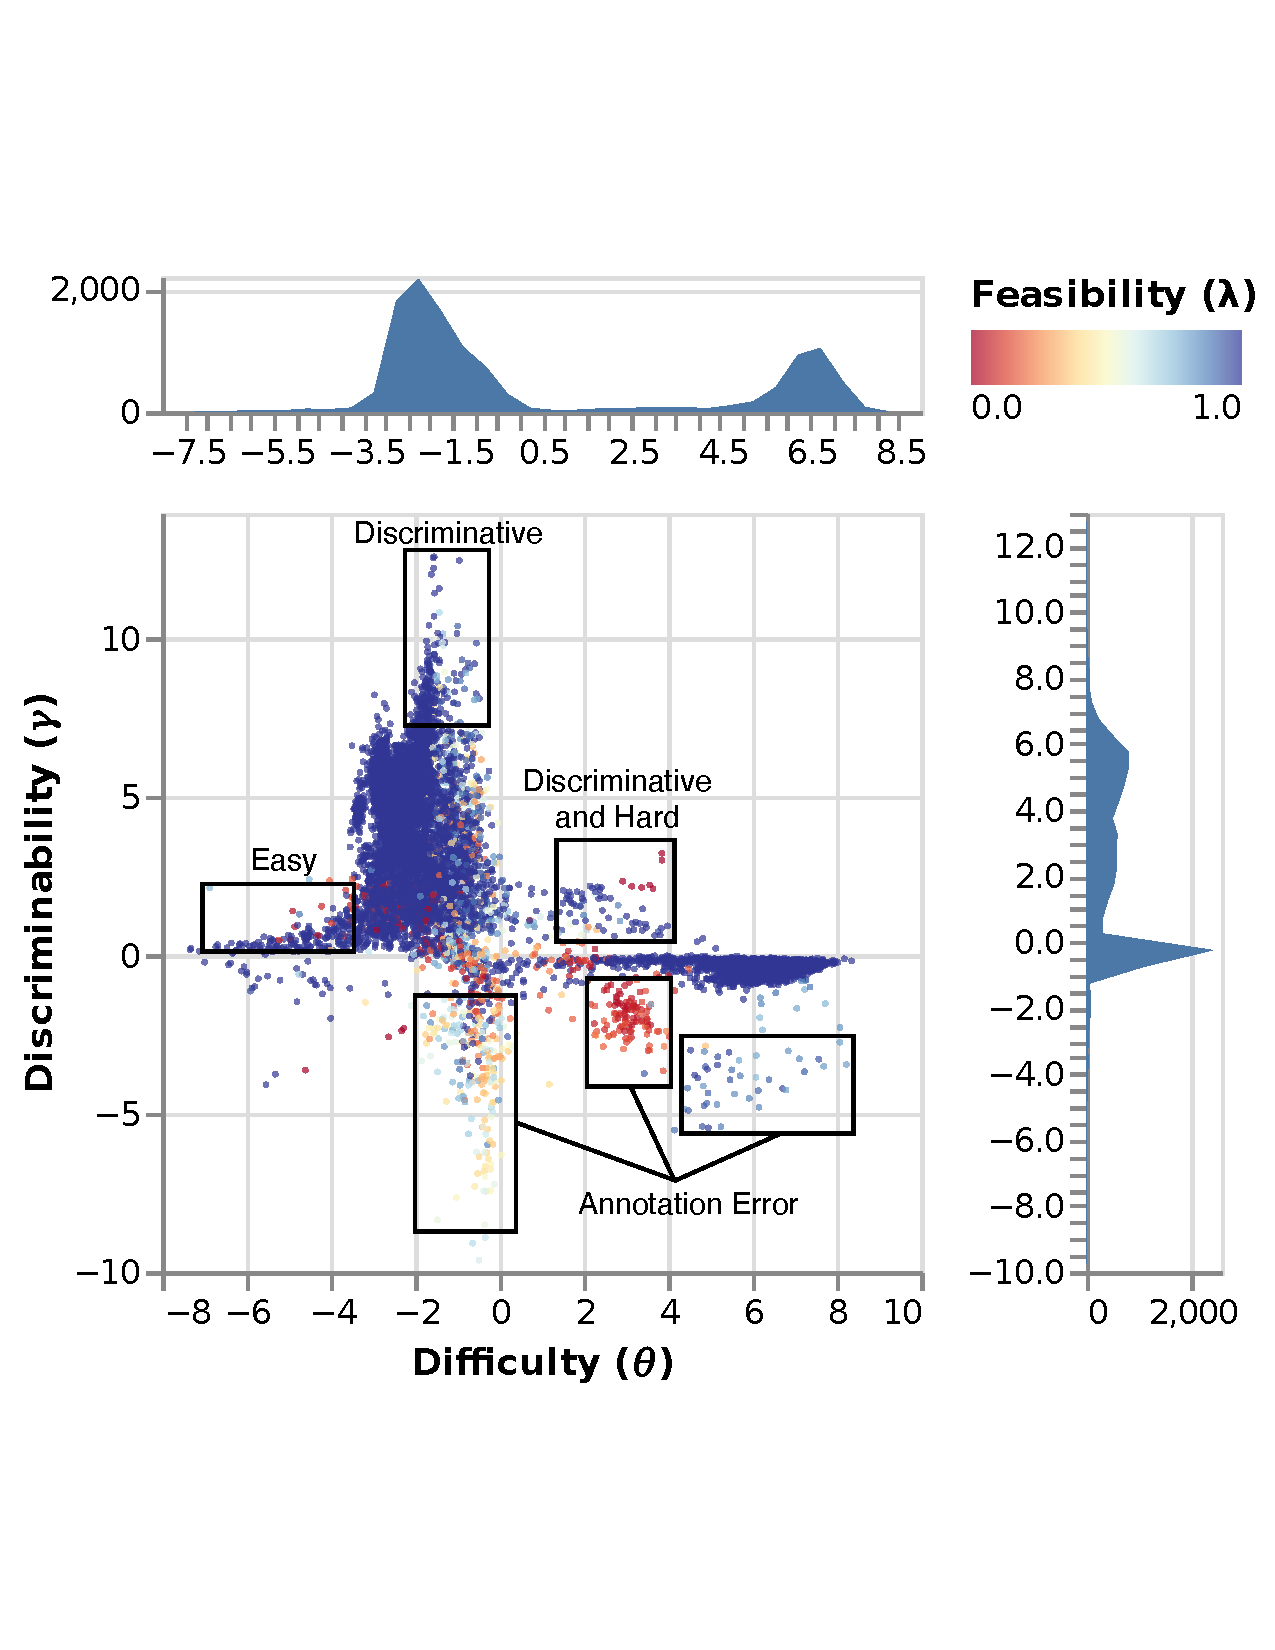
\includegraphics[width=\columnwidth]{annotated_irt_example_dist.pdf}
  \caption{
    Difficulty and Ability Discriminating (\name{}) leaderboards infer the \diff{}, discriminativeness, and feasibility of examples.
    Negative \discability{} suggests an annotation error; for example, the question with most negative \discability{}
    asks ``Why did demand for rentals decrease?'' when the answer is ``demand for higher quality housing increased.''
  }
  \label{fig:irt-dist}
\end{figure}

\subsection{How to Direct Leaderboards' Light}

To help focus attention on examples and models of interest, we propose Difficulty and Ability Discriminating (\name{}) leaderboards that explicitly model both task and submissions \emph{jointly}, rather than either in isolation.\footnote{Source code, data, and visualizations at \projecturl{}.}
%
\name{}'s underlying model is based on Item Response
Theory~\citep[\abr{irt}, reviewed in \S\ref{ch:isicle:lead}]{lord1968test,baker2001irt}, a widely used~\citep{van2016assess} alternative in educational testing to
simple
summary statistics~\citep{edgeworth1888exams}.

\name{} can explicitly identify the \emph{difficulty} and \emph{\discability{}} of \itms{} (Figure~\ref{fig:irt-dist}),\footnote{
  Example and feasibility distribution in Appendix~\ref{ch:isicle:apx:examples}.
  Interactive visualization linked from \href{https://irt.pedro.ai}{http://irt.pedro.ai}.
} which in turn can lead to a more nuanced ranking of models, identifying poor \itms{}, and better understanding of a dataset and task.
%
Throughout the paper, we use the question answering (\qa{}) benchmark \squad{}~2.0~\citep{rajpurkar2018know}.
%
For example, \name{} can identify questions that are challenging to models and questions that are wrong (incorrectly annotated).
%
In addition to better understanding datasets, it is also helpful for
efficiently selecting evaluation items to annotate.
We conclude with recommendations for future leaderboards (\S\ref{ch:isicle:conc}) and discuss where \irt{} in \nlp{} can go next (\S\ref{ch:isicle:future}).

\section{A Generative Story for Leaderboards}
\label{ch:isicle:lead}

\begin{figure}[t]
  \centering
  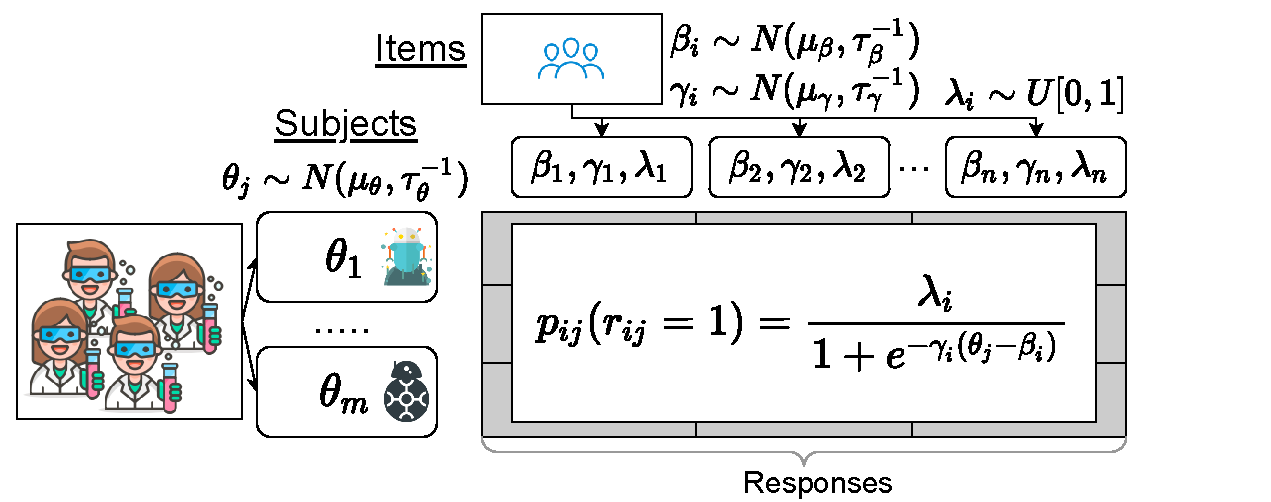
\includegraphics[width=.97\columnwidth, trim=0.5cm 0.3cm 2.6cm .4cm]{leaderboard}
  \caption{
    A \name{} leaderboard uses \irt{} to jointly infer \itm{} \diff{} $\beta_i$, \discability{} $\gamma_i$, feasibility~$\lambda_i$, and \subj{} skill $\theta_j$.
    These predict the likelihood $p_{ij}(r_{ij}=1)$ of a correct response $r_{ij}$.
  }
  \label{fig:story}
\end{figure}

Leaderboards are a product of the metrics, evaluation data, and
\subj{}s (machine or human) who answer \itms{}
(Figure~\ref{fig:story}).
%
For concreteness, let's assume that we have a question-answering task and two \subj{}s: \smart{},
who is good at trivia, and \dumb{}, who is not.
%
In the simplest \irt{} models, each \subj{}~$j$ has a random
variable~$\theta_j$ corresponding to their skill: \smart{}'s is big,
\dumb{}'s is small.

But you cannot know that until you start asking them questions of
varying \iemph{difficulty}~$\beta_i$.
%
Harder questions have a higher difficulty (``what is the airspeed of
an unladen swallow'') than easy ones (``who is buried in Grant's
tomb'').
%
The bigger the margin between a \subj{}'s skill~$\theta_j$ and an \itm{}'s
difficulty~$\beta_i$, $\theta_j-\beta_i$, the more likely that \subj{}~$j$
responds correctly~$p_{i,j}(r_{i,j}=1)$.
%
This is the simplest \abr{irt} model, which we call {\bf \pl{1}}.

Generally, given $n$ test items $\mathcal{X}=(X_1,\ldots,X_n)$
and $m$ \subj{}s
$\mathcal{S}=(S_1,\ldots,S_m)$, where each \subj{} answers every
item, we want to estimate \subj{} skills and \itm{} difficulties.
%
To discover the random variables that best explain the data, we
turn to probabilistic inference~\cite{pearl-88}.


Two additional random variables further improve \name{}:
\discability{} $\gamma_i$ and feasibility $\lambda_i$.
%
We first consider \discability{} and the margin between a
question's difficulty~$\beta_i$ and a \subj{}'s skill~$\theta_j$.
%
A discriminative question is challenging but can still be answered
correctly by a strong \subj{}.
%
If \smart{}'s ability is higher than most \itms{}' difficulty
($\theta_j-\beta_i$ is large), \itm{} discriminability multiplies this
gap by $\gamma_i$ in a model called {\bf \pl{2}}.
%
Questions with low $\gamma_i$ are low quality: they have annotation
error or do not make sense.

Another way of capturing poor quality questions is the
feasibility~$\lambda_i$.
%
For example, if the question ``who was the first president'' has the
answer \answer{Rajendra Prasad}, the question has an unstated implicit
assumption that \subjs{} must guess what country or company the
question is about.
%
In the model {\bf \pl{3}}, if a large fraction of \subj{}s all get an
\itm{} wrong, everyone's probability of getting the \itm{} right is
capped at $\lambda_i$.
%
In \nlp{} terms, $1-\lambda_i$ corresponds to the prevalence of annotation
errors that lead to unsolvable \itm{}s.


Having introduced all of the constituent elements of the model, we can
now present the full generative model:
\begin{enumerate*}
  \item For each subject $j$:
  \begin{enumerate*}
    \item Draw skill $\theta_j \sim \mathcal{N}(\mu_\theta, \tau_\theta^{-1})$
  \end{enumerate*}
  \item For each item $i$:
  \begin{enumerate*}
    \item Draw difficulty $\beta_i \sim\mathcal{N}(\mu_\beta, \tau_\beta^{-1})$
    \item Draw discriminability $\gamma_i \sim \mathcal{N}(\mu_\gamma, \tau_\gamma^{-1})$
    \item Draw feasibility $\lambda_i \sim \text{U}[0,1]$
  \end{enumerate*}
  \item Draw subject $i$ response on item $j$,\\$r_{ij} \sim p_{ij}(r_{ij} \mid \theta_j, \beta_i, \lambda_i )=$
    \begin{equation}
      p_{ij}(r_{ij}=1|\theta_j)=\frac{\lambda_i}{1+e^{-\gamma_i(\theta_j-\beta_i)}}.
      \label{eq:isicle:ours}
    \end{equation}
    For \pl{1}, $\gamma_i$ and $\lambda_i$ are fixed to 1.0, while for
    \pl{2}, only $\lambda_i$ is fixed.\footnote{In psychometrics, \pl{1}~is called a Rasch~\citep{rasch1960studies} or 1 parameter logistic (1PL) model, \pl{2}~is a 2PL model, and \pl{3}~is a 4PL model with guessing set to zero.}
\end{enumerate*}
Means $\mu_\theta,\mu_\beta,\mu_\gamma$ are drawn from
$\mathcal{N}(0,10^6)$ and $\tau_\theta,\tau_\beta,\tau_\gamma$
from a $\Gamma(1,1)$ prior, as in \citet{lalor2019latent} and
recommended by \citet{natesan2016birt}.\footnote{We differ by
  allowing $\gamma<0$ to identify bad \itms{}.  }

Because it is difficult to completely codify skill and difficulty into
a single number, we can rewrite the exponent in
Equation~\ref{eq:isicle:ours} as a sum over dimensions
$-\gamma_i(\sum_k \bm{\theta}_{j,k}-\bm{\beta}_{i,k})$,
where each dimension captures the interaction between an \itm{}'s
difficulty and a \subj{}'s skill.
%
For example, perhaps \dumb{} could better exploit artifacts in one
dimension (their skill for $\theta_{j,k=5}$ is high but everywhere
else is low) while \smart{} might not know much about a particular
topic like potent potables ($\theta_{j,k=2}$ is low but everywhere
else is high).
%
We call this model {\bf \pl{m}}.\footnote{
  We do not incorporate feasibility into the \pl{m}~model since it already improves over 1D models without it.
}
%
Multidimensional \irt{} models~\citep{reckase2009mirt} could---in addition to better modeling
difficulty---also cluster items for interpretation; we briefly
experiment with this (Appendix~\ref{ch:isicle:clustering}), but leave
more to future work (\S\ref{ch:isicle:future}).

\subsection{Examples are Not Equally Useful}

\irt{}'s fundamental assumption is that not all \itms{} and
\subjs{} are equal.
This explains why leaderboards can fail while having
``normal looking'' accuracies.
%
As a thought experiment, consider a dataset that is one third easy
($\beta_i \in [0,1]$), one third medium difficulty
($\beta_i \in [2,3]$), and one third hard ($\beta_i \in [6,7]$).
%
Suppose that \smart{} has skill $\theta_{k}=4$ while \dumb{} has skill
$\theta_{b}= 2$.
%
A standard leaderboard would say that \smart{} has higher accuracy
than \dumb{}.
%
But suppose there's a new \subj{} that wants to challenge \smart{};
they are not going to reliably dethrone \smart{} until their skill
$\theta_{c}$ is greater than six.

This is a more mathematical formulation of the ``easy'' and ``hard''
dataset splits in question
answering~\citep{sugawara2018easier,Rondeau2018-um,sen2020learn}.
%
In \pl{3}, this recapitulates the observation of
\citet{boydgraber2020nerds} that annotation error can hinder effective
leaderboards.
%
\name{} helps systematize these observations and diagnose dataset issues.


\subsection{Inference}

To estimate the latent parameters of our model, we use mean-field
variational inference~\cite{jordan-99}.
%
In variational inference, we propose a distribution over the latent
variables,~$q_\phi(\cdot)$, that approximates the true but intractable
posterior~$p(\cdot)$.
%
We then minimize the \abr{kl}-divergence between these distributions,
equivalent to maximizing the evidence lower-bound (\textsc{elbo}) with
respect to the variational parameters.

In our case, $q_\phi(\cdot)$ is a mean-field distribution, which means it
factorizes over each of the latent variables (the product is over the
$n \times m$ subject-item pairs)
\begin{align*}
  q_\phi(\bm{\theta}, \bm{\beta}, \bm{\gamma}, \bm{\mu}, \bm{\tau}) = q(\bm{\mu})q(\bm{\tau})\prod_{i,j} q(\theta_j)q(\beta_i)q(\gamma_i)
\end{align*}
Specifically, for our key latent variables $z \in \{\bm{\theta}, \bm{\beta}, \bm{\gamma}\}$, the associated variational distributions are of the form $q(z) = \mathcal{N}(u_z, t_z^{-1})$.
Recall that in the generative distribution, each latent $z$ is drawn from a $\mathcal{N}(\mu_z, \tau_z^{-1})$ whose parameters are also latent variables; for these variables, we use the variational distributions $q(\mu_z) = \mathcal{N}(u_{\mu_z}, t_{\mu_z}^{-1})$ and $q(\tau_z) = \Gamma(a_{\tau_z}, b_{\tau_z})$. We optimize the \textsc{elbo} with respect to the variational parameters
\begin{align*}
  \bm{\phi} & =\{\bm{u}_z,\bm{t}_z,\bm{u}_{\mu_z},\bm{t}_{\mu_z},\bm{a}_{\tau_z},\bm{b}_{\tau_z},\bm{\lambda}\}
\end{align*}
for all $z$ using \abr{adam}~\citep{Kingma2014AdamAM}.

With \name{}'s leaderboard \irt{} model introduced, we next discuss
how leaderboard \subj{}s are statistically compared and alternative
methods---such as using \irt{} parameters---to evaluate whether two
models are truly different.

\section{Ranking and Comparing Subjects}
\label{ch:isicle:compare}

% Doesn't seem to fit either the previous or the next section.
% I see the point about short section, don't see an obviously better soln
%\jbgcomment{Should this be it's own section or be demoted to subsection?}

Fundamentally, the objective of comparative evaluations like
leaderboards is to decide whether model~$A$ is better than model~$B$.
%
A thread of \nlp{} has rightfully advocated for adding rigor to these
decisions using statistics~\citep[Classical Testing
  Theory]{traub1997ctt} where the objective is to infer a true
score~$T$ from the observed test score~$X=T+E$ given a measurement
error~$E$, uniform across \subj{}s.
%
However, in educational testing---a field measuring skill and
knowledge in humans---\irt{} is a primary measurement
instrument~\citep[p.~2]{hambleton1991fundamentals}.
%
A major motivation for \irt{} is that \subj{}s of different skill have
\iemph{different} errors.
\irt{} explicitly accounts for the bandwidth-fidelity
dilemma~\citep{mcbride1976bandwidth}: \itms{} can either accurately
measure a narrow ability range (fidelity) \textit{or} inaccurately
measure large ability ranges (bandwidth).\footnote{Estimation error
  of $\theta$ varies by position (Appendix~\ref{ch:isicle:irt-test}).  }
%
This section and the next contrast methods for identifying the best
model and advocate for \irt{}.

% \subsection{Classical Ranking by Aggregated Metrics}
\label{ch:isicle:agg}

%\jbgcomment{This might also be demoted}

Implicit in nearly all leaderboard evaluations is ranking models by a
statistic such as the average accuracy.
As we show in \S\ref{ch:isicle:exp}, na\"ive rankings are noisier than \irt{} rankings.

\section{IRT for Leaderboards}
\label{ch:isicle:exp}

Leaderboards should: (1) reliably and efficiently rank
better models ahead of worse
models~\citep{sutcliffe1992pragmatics,voorhees2003evaluating} and (2)
guide inspection of \itms{} and \subjs{} (\S\ref{ch:isicle:interp}).
%
The first ameliorates the unavoidable randomness
of finite evaluations while the second enables
error analysis~\citep{wu2019errudite} and model
probing~\citep{belinkov2019survey,zhang2019manifold}.
%
First we verify that \irt{} models accurately predict the \resps{} of
\subjs{} (\S\ref{ch:isicle:irt-accurate}).
%
Next, a ranking stability analysis shows that \irt{} has
modestly better reliability than classical rankings
(\S\ref{ch:isicle:irt-compare}).
%
Lastly, using \irt{} to actively sample \itms{} for annotation yields
rankings with better correlation to complete test data
(\S\ref{ch:isicle:sampling}).

\subsection{Why a Linear Model Baseline}

At first blush, the differences between \irt{} and logistic regression
are minimal, but we include the comparison to address natural
questions from the \abr{nlp} community:
%
(1) do the idiosyncrasies of the \irt{} formulation hurt
accuracy?
%
(2) should we add features to better understand phenomena
in the questions?
%
(3) why not use deep models?

The next section argues that both \irt{} and logistic regression are
accurate even without laboriously engineered task-specific features.
%
Adding obvious features such as \itm{} words (e.g., questions)
only minimally improves the accuracy.
%
We explicitly omit less interpretable deep models since our goal is to
make leaderboards \emph{more} interpretable.

\subsection{Response Prediction is Accurate}
\label{ch:isicle:irt-accurate}

Just as educational testing researchers validate \irt{} models by
seeing if they predict \subj{} \resps{}
correctly~\citep{aera2014standards}, we validate how well \name{} predicts
whether \squad{} models get questions right.

We compare against a logistic regression linear model (\abr{lm})
implemented with Vowpal Wabbit~\citep{Agarwal2014ARE}.
%
Since integrating hand-crafted features is easy, we incorporate
features derived from \subj{} \abr{id}s; \itm{} \abr{id}s; functions
of the \squad{} question, answer, and title; and \irt{} parameters
(details in Appendix~\ref{ch:isicle:apx:features}).
%
As in \irt{}, logistic regression predicts whether a \subj{} correctly
responds to an \itm{}.
%
Later, we discuss ways to integrate more features into \irt{}
(\S\ref{ch:isicle:future}).

\subsubsection{SQuAD Leaderboard Data}
\label{ch:isicle:datasets}
Experiments are on the \squad{} 2.0 leaderboard.
Development data are publicly available, and organizers provide test set responses.
There are $161$ development \subjs{}, $115$ test \subjs{}, and \num[group-separator={,}]{11873} \itms{} ($1.9$ million total pairs).
Experiments that do not need test responses use all development \subjs{}; those that do use the smaller test subset.

\subsubsection{Evaluation Scheme}

Following prior work~\citep{wu2020virt}, we evaluate \irt{} and linear models by holding out 10\% of responses and computing classification metrics.\footnote{Everywhere else in the paper, we train on all responses.}
%
In \squad{}, predicting whether a \resp{} is correct is an imbalanced
classification problem (80.4\% of responses in the development set are
correct).
%
Thus, we use \abr{roc auc}, macro F1, and accuracy.

\subsubsection{IRT Response Prediction is Accurate}
\label{ch:isicle:irt-compare}

\irt{} models that incorporate more priors into the generative story should be better, but are they?
We compare four \irt{} models: \pl{1}, \pl{2}, \pl{3}, and \pl{m}~(\S\ref{ch:isicle:lead}).
The more sophisticated models are better and all improve over the
\abr{lm} (Figure~\ref{fig:vw-ablation}) and correlate well with each other (Appendix~\ref{apx:irt-self-corr}).
To be clear, while higher accuracy than \abr{lm} is good, our goal is to validate that \irt{} models are accurate; later, we inspect model errors and identify annotation errors (\S\ref{ch:isicle:interp}).

\begin{figure*}[th]
    \centering
    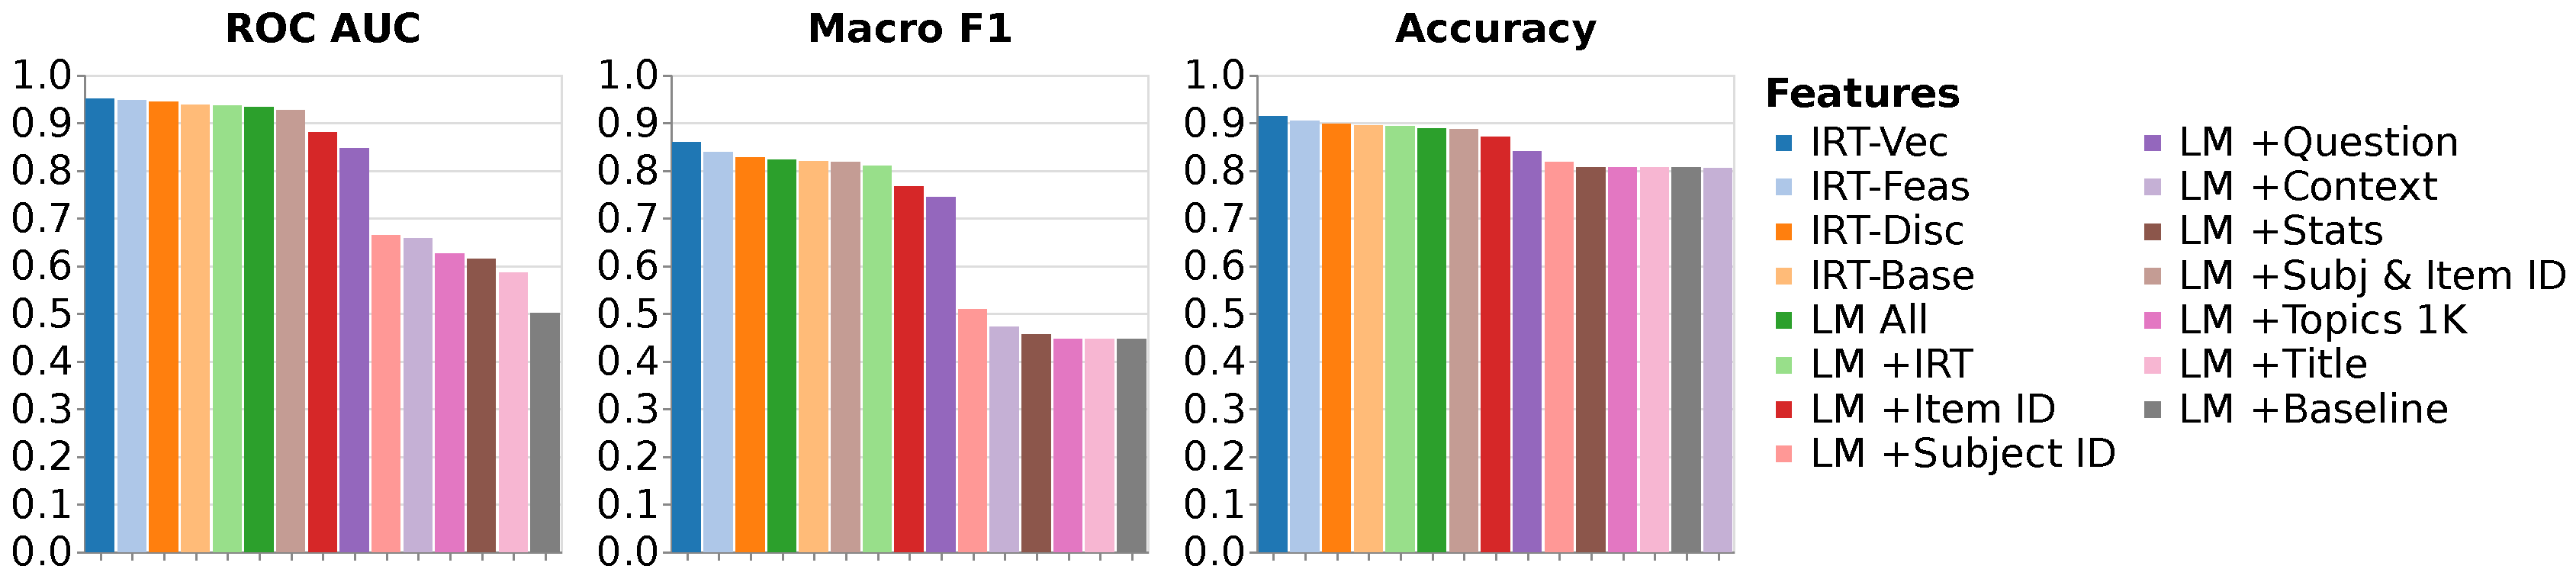
\includegraphics[width=\textwidth]{vw_ablation}
    \caption{
        We compare each \irt{} and linear model (\abr{lm}) by how well they predict \subj{} \resps{}.
        We focus on \abr{roc auc} since predicting responses is an imbalanced classification problem (most \subjs{} are correct).
        Under that metric, all \irt{} models improve over the best
        \abr{lm}, and the strongest \abr{lm} ablation only uses \irt{} features.
        That textual features are predictive in the \abr{lm} suggests they could improve future models.
    }
    \label{fig:vw-ablation}
\end{figure*}


\subsubsection{What Model Features are Predictive?}

Integrating additional features into Bayesian models is not trivial,
so we instead use the flexibility of linear models to identify useful
features.
%
Our leave-one-in ablation compares features (Figure~\ref{fig:vw-ablation}):
the top ablations both use \irt{} features, further validating
\irt{} parameters.
%
The \subj{} and \itm{} identifier features are also
strongly predictive, but \itm{} is the stronger of the two.
%
Text-based features are weaker, but this suggests future work to
better integrate them into \irt{} models (\S\ref{ch:isicle:future}).



\subsection{Ranking with IRT}

Leaderboards should produce \iemph{reliable} \subj{} rankings: can
\name{} rank systems even with a tiny test set?
%
Thus, we compare the correlation both of traditional average accuracy
(\S\ref{ch:isicle:agg}) and \irt{} rankings on the whole test
set compared to the rankings of the same metric on a smaller test set.
%
Our first experiment (\S\ref{ch:isicle:stable}) examines the stability
of existing \itms{} and \subjs{} while the second
(\S\ref{ch:isicle:sampling}) investigates stability of ``new''
evaluation data using sampling strategies.

\subsubsection{IRT Rankings Have Better Reliability}
\label{ch:isicle:stable}

\begin{figure*}[t]
    \centering
    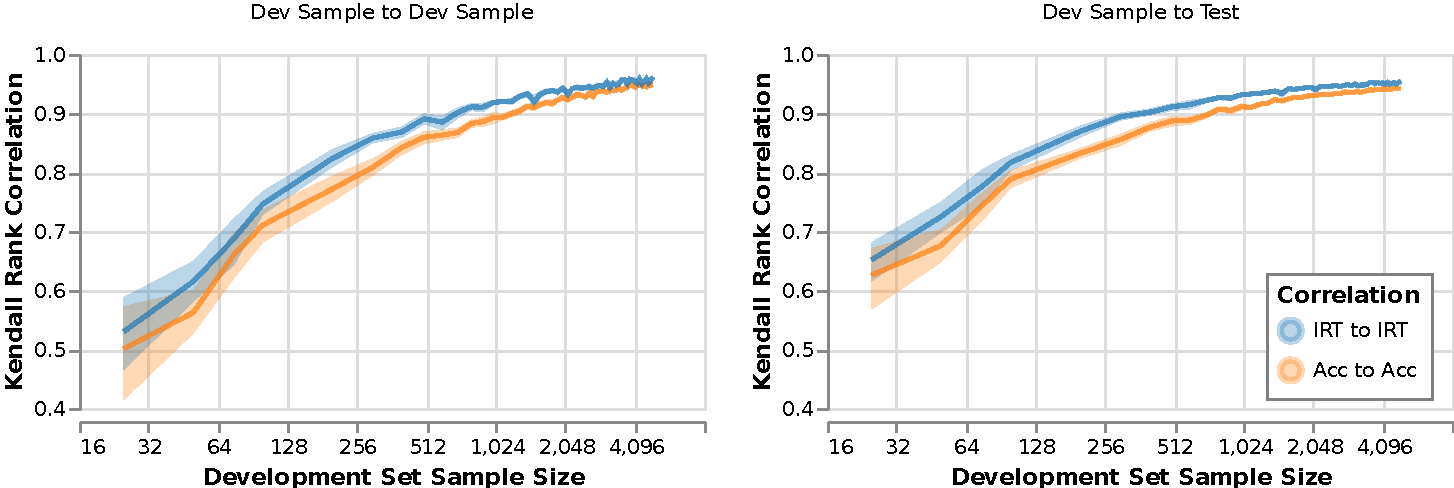
\includegraphics[width=\textwidth]{stability_simulation_corr}
    \caption{
        Compared to the final ranking over a large test set, how well does a small test set correlate?
        %
        The left shows correlation between mutually exclusive development set samples and the right between development samples and the full test set.
        %
        In both experiments (panes), ranking systems by \irt{} ability is more stable---across all sample sizes---than mean accuracy and thus more reliable (Kendall's rank correlation is higher).
        %
        Bands show 95\% confidence intervals of rank correlations across ten trials per sample size.
    }
    \label{fig:stability}
\end{figure*}

Rankings should be reliable within the same dataset (e.g., on dev
set) and generalize to similar datasets (e.g., with a test dataset).
%
To test the first, we measure the ranking stability of mutually
exclusive samples of the development
data~\cite{buckley2000measure}.
%
To test the second, we measure the correlation between
development set sample rankings to test set rankings~\citep{voorhees1998var}.

Specifically, for a range of sample sizes\footnote{ The sample size
    must be less than half the size of the development data so that we
    can obtain two samples.  } we (1) sample two partitions of the data,
(2) compute the classical ranking\footnote{For \squad{}, ordering by
    mean exact match score.} and the \irt{} ranking from a refit
\pl{3}~model, then (3) compute Kendall's
correlation~\citep{kendall1938tau} between the samples for each
ranking (details in Appendix~\ref{ch:isicle:apx:rank-stability}).
%
In both cases \irt{} rankings have higher correlation than classical
rankings (Figure~\ref{fig:stability}, left).
%
Since the benefit is strongest at low sample sizes, \irt{} can improve
the reliability of small-scale evaluations.
% Checking for ranking stability assesses the degree to which noise from data collection affects reliability, but does not address how good a predictor development performance is of test performance.

The second experiment examines ranking generalization: \irt{} yields more reliable measures of \subj{} skill,  implying a greater consistency in subject rankings across evaluation settings.
Figure~\ref{fig:stability} compares the development set sample rankings computed above to rankings obtained using subjects' \emph{test} set responses (with the same \irt{} model).

Across all sample sizes, subjects' \irt{} ability estimated on the
development set correlates well test set ability.
%
Crucially, this is better than the corresponding classical metrics
like accuracy (Appendix~\ref{ch:isicle:apx:rank-stability} quantifies
the statistical significance of the difference), supporting our
original motivation for using \irt{}.\footnote{ Since the maximum trial size was
    limited, we train one final model with the full data, see
    Table~\ref{tab:rank-corr} in the
    Appendix~\ref{ch:isicle:apx:rank-stability}.  }

\subsection{IRT Improves Cold Start Reliability}
\label{ch:isicle:sampling}

\irt{} can also guide the construction of tests.
Just as \irt{} practitioners prepare tests for humans, we too construct tests for machines.
In educational testing, collecting responses from humans is expensive; likewise, although \emph{questions} are cheap in search-based \qa{} tasks~\citep{Nguyen2016MSMA,kwiatkowski2019nq}, annotating \emph{answers} is expensive.
Likewise, ``grading'' machine dialog responses is expensive and \irt{} helps~\citep{sedoc2020irt}.
To emulate this setting, we use computerized adaptive testing~\citep{weiss1984cat} to iteratively select \squad{} \itms{} to ``annotate.''

As in human test preparation, we use existing annotations to infer
\itm{} parameters and iteratively infer the ability of new \subjs{}.
%
This experiment splits~$m$ \subjs{} into a training group (80\%) and a
testing group (20\%).
%
The training group represents \subjs{} for which we have full \itm{}
predictions and annotations; the testing group represents a new group
of \subjs{} that we need to rank.
To efficiently rank, we should iteratively choose \itms{} to annotate that yield the most information about the ranking if all the data were annotated.

This experiment compares how well several \itm{} selection strategies work.
For each selection method, we (1) choose a sample size, (2), sample
from the development set, (3) compute the ranking of \subjs{}, and (4)
compute Kendall's rank correlation
(Figure~\ref{fig:stability:sampling}).\footnote{We compute correlations with the complete development set on ten trials to build $95\%$ confidence intervals.}


\begin{figure}[t]
    \centering
    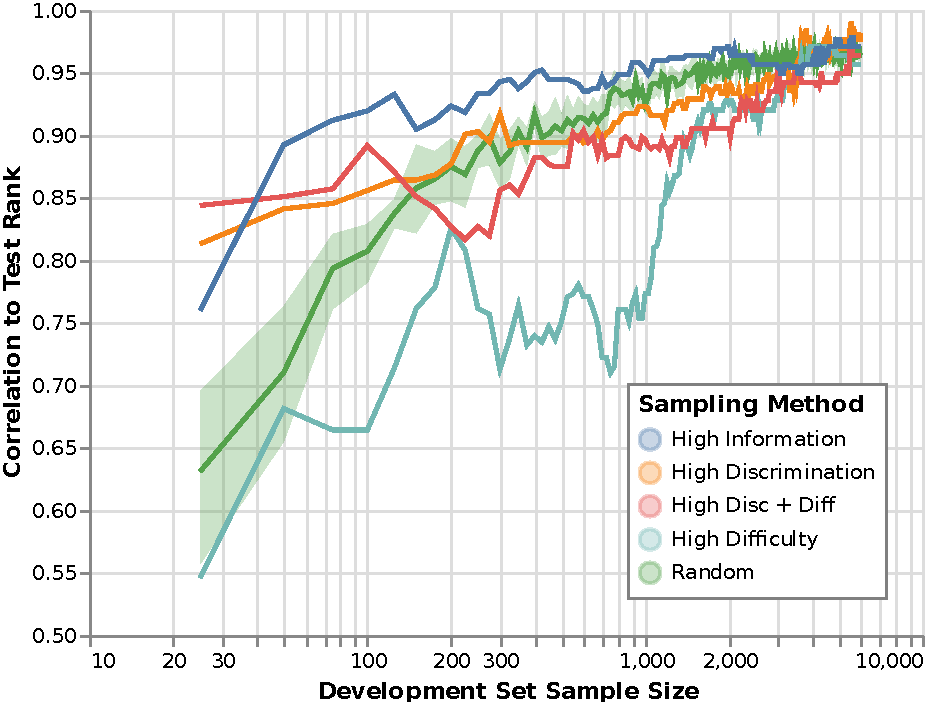
\includegraphics[width=\columnwidth]{cat_sampling_rank}
    \caption{
        Suppose we need to cold start and collect annotations for a new \subj{}: what order would most rapidly increase correlation to the full test data?
        As we expect, the correlations eventually converge, but with little data, \irt{} has better correlation than other methods.
        We suspect that the \irt{} information underperforms early on
        when the \subj{} ability estimate is unstable.
    }
    \label{fig:stability:sampling}
\end{figure}

% \jbgcomment{Below paragraph needs more intuition (both overall and for
%   the equation).  Currently, this is also stuck at the top of a page
%   in my compile, would be good to unpin it so that we don't have
%   widow.}

Which \itm{} selection strategies should we compare?
As a baseline, we use na\"ive random sampling.
Like prior work, we compare selecting \itms{} with the highest \diff{} and the highest \discability{}~\citep{lalor2019latent} as well as the sum of the two.\footnote{We train an \pl{2}~model to simplify sampling (e.g., avoiding a tradeoff between feasibility and \discability{}).}
We propose that \itms{} should be selected according to their Fisher information content~\citep{weiss1982info}
\begin{equation}
    \label{eq:info}
    I_i(\theta_j)=\frac{(p_{ij}')^2}{p_{ij}(1-p_{ij})}=\gamma_i^2 p_{ij}(1-p_{ij})
\end{equation} as derived by \citet[p. 70]{lord1968test}.

Intuitively, if we do not yet know the true skill~$\theta_j$, we should pick \itms{} whose expected response we are most uncertain about.
Our uncertainty (entropy) is maximized when the likelihood of a correct response $p_{ij}$ is the same as the likelihood of an incorrect response $1-p_{ij}$, which corresponds to the maximal value of $I_i(\theta_j)$; it is also sensible this value increases as \discability{} $\gamma_i$ increases.

To infer the maximally informative \itms{}, we estimate the ability
$\theta_j$ of each \subj{} using the currently selected \itms{}, use
the ability to compute the information
of each yet-to-be-annotated \itm{} for each \subj{}, and then aggregate the informativeness
\begin{equation}
    \text{Info}(i)=\sum_j I_i(\theta_j)
\end{equation}
by \itm{}~$i$ summed over \subjs{}~$j$.
This approach is similar to uncertainty sampling and reduces to it for the \pl{1}~model~\citep{lewis1994uncertainty}.
We initially seed with the twenty-five most discriminative \itms{} (details in Appendix~\ref{ch:isicle:apx:rank-stability}).

Like computerized adaptive testing~\citep{moreno1984cat}, Figure~\ref{fig:stability:sampling} shows that at lower sample sizes three of the \irt{} sampling methods are better than random sampling---\diff{} does worse.
The other \irt{} methods have comparable correlation.
Thus, by using \irt{}, \name{} can both improve rankings and guide annotation.

\section{Qualitative Insights on Leaderboards}
\label{ch:isicle:interp}

\name{} also helps qualitative analysis of \itms{} and \subjs{}.
First, \irt{} identifies overfitting and generalizes partitioning datasets by \diff{}.
Then we show that---like in educational testing---\irt{} identifies good and bad \itms{}.

\subsection{Guiding Analysis with IRT}

\begin{figure*}[t]
    \centering
    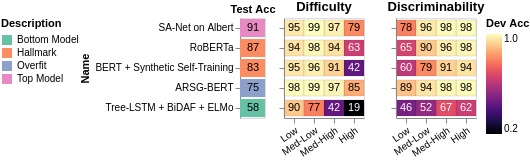
\includegraphics[width=.8\textwidth]{irt_confusion}
    \caption{
        We partition evaluation data by \irt{} \diff{} and
        \discability{} with accuracy in each quartile.
        Most improvements in high-accuracy systems come from getting
        high-difficulty questions right.
        \Itms{} with low \discability{} (and thus prone to annotation errors) are difficult for all \subjs{} except the overfit \abr{args-bert} model.
        We include top-performing \squad{} \subjs{}, several notable
        \subjs{} (systems), and a pair from the bottom of the leaderboard.
    }
    \label{fig:confusion}
\end{figure*}

Several works curate easy and hard \abr{qa} subsets based on how many
models answer correctly~\citep{Rondeau2018-um} or
heuristics~\citep{sugawara2018easier}.
%
\irt{} can create similar subsets using \pl{3}, the best 1D model.
%
\Diff{} finds where \subjs{} improve while \discability{} and
feasibility can surface \itms{} that may be invalid.
%
For example, one low feasibility question (Figure~\ref{fig:ex-feas}) asks
``what are two examples of types of Turing machines?'' which has two
problems: (1) the answer omits five types and (2) span-based
evaluation precludes selecting non-contiguous types.
%\jbgcomment{What's a combination of types?  Or is this just more than one type?}

After excluding \itms{} with negative \discability{}---they are
likely erroneous---we sort \itms{} into bins.
%
We break both \diff{} and \discability{} into four bins---taking the 25\textsuperscript{th},
50\textsuperscript{th}, and 75\textsuperscript{th}
percentiles---creating eight total bins.
%
Then we select representative \squad{} \subjs{} with their
exact match scores (Figure~\ref{fig:confusion}).
%
Let's examine a feasible \itm{} with positive \diff{} and \discability{} like ``what reform was attempted following the Nice treaty?''\footnote{
    A: ``there was an attempt to reform the constitutional law of the \abr{eu} and make it more transparent.'' (Appendix Figure~\ref{fig:ex-reasonable})
}
In this case, the annotator's span is too long---resulting in almost
no correct answers and a low fuzzy match (token F1).
%
In contrast, one highly discriminative question succeeds because there
are multiple plausible guesses to ``who did the Normans team up with
in Anatolia?''\footnote{ Example with statistics in Appendix
    Figure~\ref{fig:ex-tricky}.
}
While both \answer{the Armenian state} and \answer{Turkish forces} are
superficially plausible answers, only \answer{Turkish forces} is correct;
nonetheless, some models are fooled.
%
Using \irt{} to guide \subj{} analysis is helpful; next, we test how
efficient it is in identifying annotation error.

\subsection{Identifying Annotation Error}

To test if \irt{} can identify annotation error, we inspect sixty \squad{} development set \itms{}.
We select ten \itms{} from each of these groups: the most negative \discability{}, \discability{} nearest to zero, the highest \discability{}, the least difficult, most difficult, and \irt{} model errors.
For each, we annotate whether the \itm{} was correct, was ``correct'' yet flawed in some way, or simply wrong (Figure~\ref{fig:example-error}).\footnote{
    Annotation guidelines provided in supplementary materials; Figure~\ref{fig:example-error} uses the first set of annotations which were later augmented by two additional sets of annotations.
}
%
Inter-annotator agreement between three authors on this three-way annotation with Krippendorff's $\alpha$~\citep{kripp2004,artstein2008inter} is $0.344$.
%
Despite only modest agreement, just as in the development of education tests, negative \discability{} is predictive of bad \itms{}.
%
When \discability{} is negative, then the probability of getting
the answer right is higher when ability is \emph{lower}, which is
undesirable: \smart{} consistently loses to \dumb{} on those \itms{}.
%
This could identify bad \itms{} in evaluation sets for removal.
%\jbgcomment{Expand on this a little bit}
\begin{figure*}[t]
    \centering
    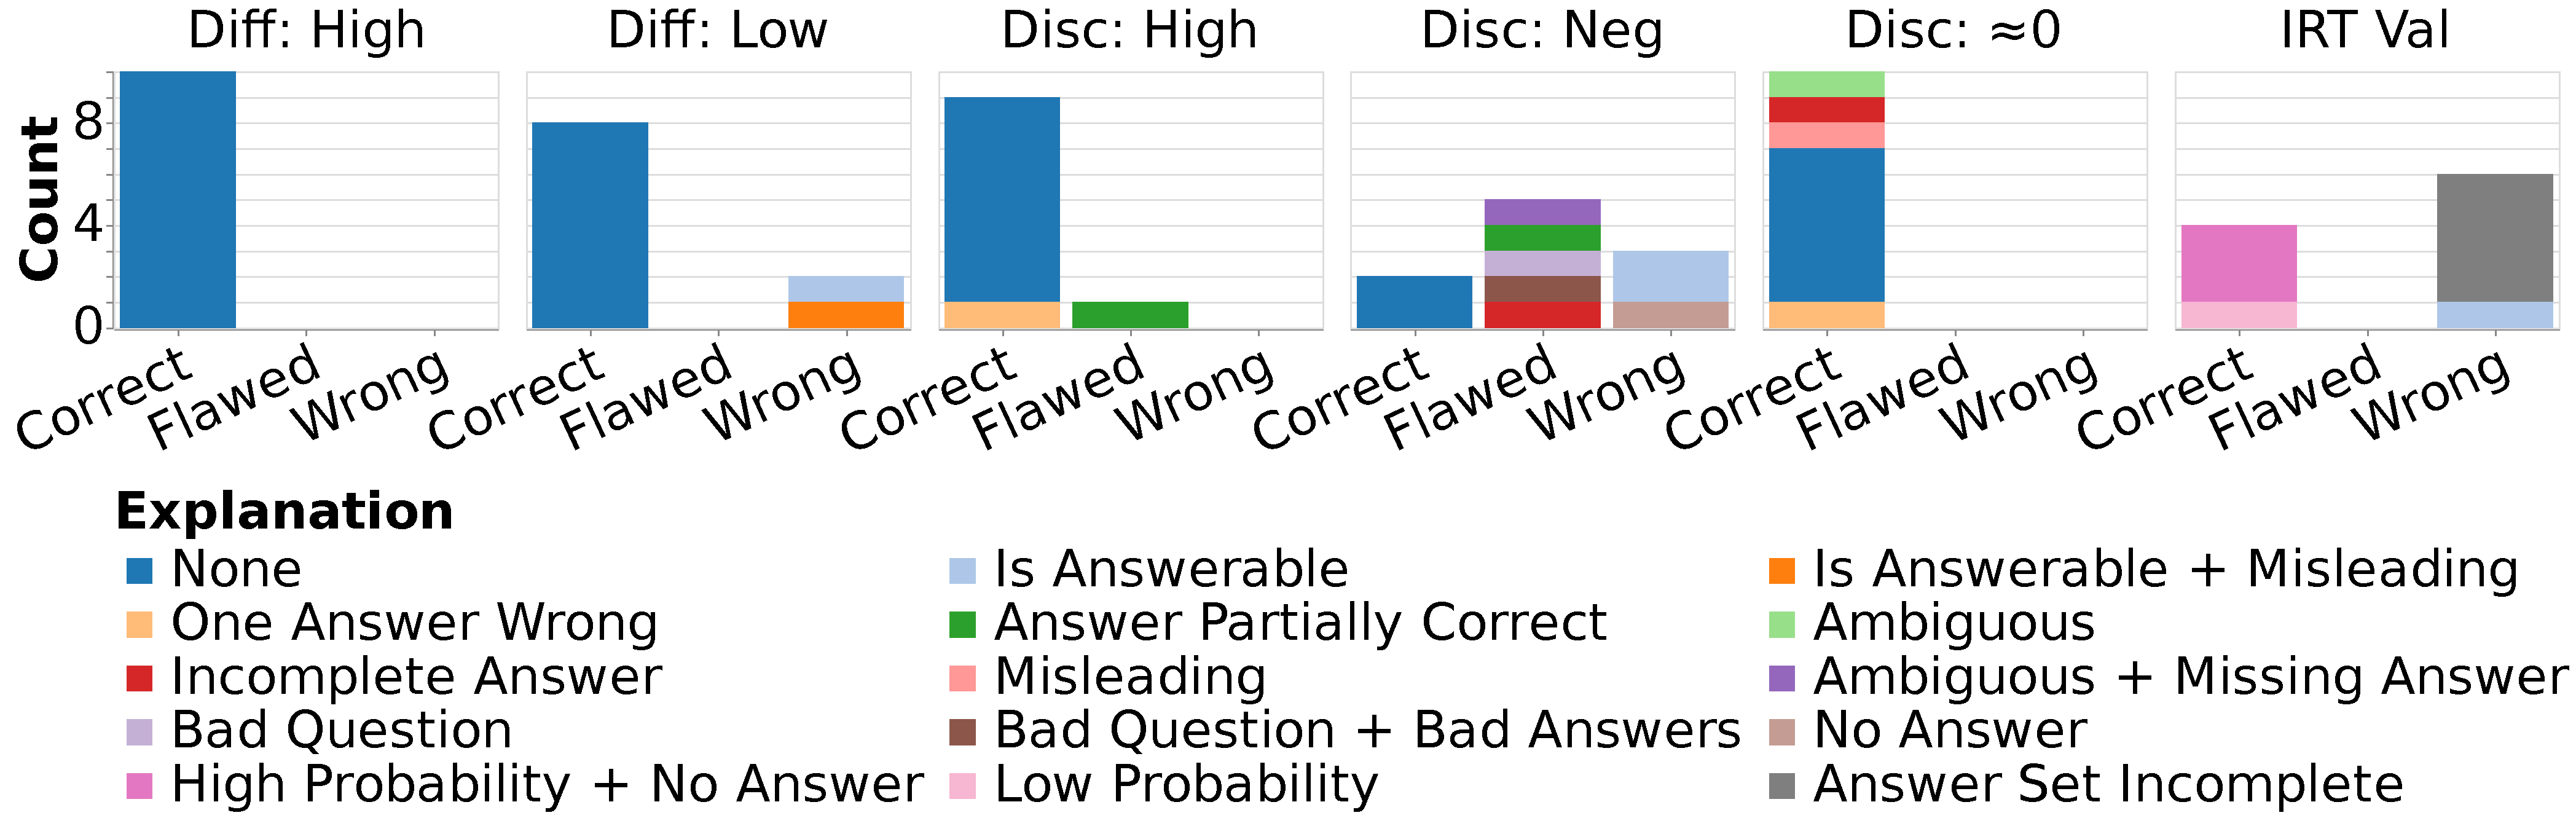
\includegraphics[width=\textwidth]{example_analysis.pdf}
    \caption{
        We annotate \squad{} \itms{} by \discability{}, \diff{}, and \irt{} prediction errors.
        For example, one question with negative \discability{} was classified as ``Wrong'' with the explanation that the annotated answer indicates it is \iemph{not} answerable, but the question actually \iemph{is} answerable.
        \Itms{} with negative \discability{} or where \irt{}'s prediction is wrong have a much higher rate of annotation error (``Flawed'' or ``Wrong'').
        Using similar methodology, errors in datasets could be more rapidly identified.
    }
    \label{fig:example-error}
\end{figure*}

\section{Related Work}
\label{ch:isicle:rel}

\name{} draws together two primary threads: we use \irt{} to
understand datasets, which has been applied to other \abr{nlp} tasks,
and apply it to improving leaderboards.
%
%In this section and the next we review alternative applications of \irt{} in \abr{nlp} and alternative approaches for improving leaderboards.
%
Finally, we explore how the insights of \irt{} can improve not just
the analysis of test sets but to improve the \emph{construction} of
test sets.

\paragraph{\textbf{\abr{irt} in \abr{nlp}}}
\irt{} is gaining traction in machine learning
research~\citep{martinez2016ml,martinez2019irt} where automated metrics can be
misleading~\citep{sedoc2019chateval}: machine
translation~\citep{hopkins2013competitions} and chatbot
evaluation~\citep{sedoc2020irt}.
%
Concurrent with our work, \citet{vania2021compare} compare \nlp{} test sets with \irt{}.
Closest to our work in \nlp{} is \citet{otani2016aggregation}, who
rank machine translation \subjs{} and compute correlations with gold
scores.  Similarly, \citet{martinez2020indicators} use \irt{} on
non-language \abr{ai} video game benchmarks.
%
Just as we use \irt{} to identify difficult or easy \itms{},
\citet{lalor2016irt} create challenge sets for textual entailment.
%
We
test \irt{} as a way to guide annotation, but it can also
train \nlp{} models; for example, deep models learn ``easy'' examples
faster~\citep{lalor2018diff} and maintain test accuracy when training
data are down-sampled~\citep{lalor2019latent}.

\paragraph{\textbf{Improving Leaderboards}}
%
The rise \nlp{} leaderboards has encouraged critical thought into
improving them~\citep{linzen2020progress}, improving evaluation more
broadly~\citep{eger2020workshop}, and thoughtful consideration of
their influence on the direction of
research~\citep{sculley2018curse,dotan2020value}.
%
\name{} aims make leaderboard
yardsticks~\citep{hernandez2020yardsticks} more reliable,
interpretable, and part of curating the benchmark itself.
%
In line
with our reliability goal, just as statistical tests should appear in
publications~\citep{dror2018guide,Dodge2019ShowYW}, they should be
``freebies'' for leaderboard
participants~\citep{ethayarajh2020utility}.  Alternatively,
\citet{hou2019leader} posit that leaderboards could be automatically
extracted from publications.
%
How to aggregate multi-task
benchmarks~\citep{wang2018glue,wang2019superglue,fisch2019mrqa} and multi-metric benchmarks~\citep{ma2021dynaboard} is an
open question which---although we do not address---is one use for
\irt{}.


This work implicitly argues that leaderboards should be
continually updated.  As a (static) leaderboard ages, the task(s)
overfit~\citep{recht2019generalize} which---although
mitigable~\citep{blum2015ladder,andersonCook2019host}---is best solved
by continually collecting new data~\citep{kiela2021dynabench}.
%
Ideally, new data should challenge models through adversarial
collection~\citep{wallace2018trick,nie2019adversarial} and related
methods~\citep{Gardner2020-gn}.  However, if making an easy
leaderboard more difficult is possible, the
leaderboard has outlived its helpfulness and should be retired~\citep{voorhees1999trec8}.

Part of our work centers on alternate task efficacy rankings, but this
na\"ively assumes that task efficacy is the sole use case of
leaderboards.
%
Indeed, focusing solely these factors can mislead the
public~\citep{paullada2020data} and may not reflect human language
capabilities~\citep{schlangen2020targeting}.
%
Leaderboards are also well positioned to provide incentive structures
for participants to prioritize fairness~\citep{bender2018data} and
efficiency~\citep{strubell2019energy,schwartz2020green,min2021efficientqa}
or incorporate testing of specific
capabilities~\citep{ribeiro2020checklist,Dunietz2020-ty}.
%
To enable these more nuanced analyses, leaderboards should accept
runnable models rather than static
predictions~\citep{ma2021dynaboard}.

\paragraph{\textbf{Active Learning}}
Beyond \irt{}, the analysis of training dynamics and active learning~\citep{settles09active} is helpful for actively sampling specific \itms{} or identifying low-quality \itms{}~\citep{brodley1999mislabel}.
For example, \citet{swayamdipta2020cartography} and \citet{pleiss2020aum} propose alternative training dynamics-based methods for identifying difficult \itms{} as well annotation errors.
Even closer to goals, \citet{rahman2020active} use active learning to build a test collection.
%
Explicitly measuring how effectively examples separate the best \subj{} from the rest allows test set curators to ``focus on the bubble''~\citep{boydgraber2020nerds}, prioritizing examples most likely to reveal interesting distinctions between submitted systems.
%
%Generally, the family of uncertainty sampling methods~\citep{lewis1994uncertainty} are similar to maximizing item information (\S\ref{ch:isicle:sampling}), but our primary application is towards collecting evaluation data rather than training \nlp{} models.

\paragraph{\textbf{Alternate Formulations}}
%
\irt{} is an example of convergent evolution of models that
predict \subj{} action given an \itm{}.
%
Ideal point models~\cite{poole2017voting} consider how a legislator (\subj{})
will vote on a bill (\itm{}) and use a similar mathematical formulation.
%
The venerable \abr{elo} model~\cite{glickman-99} and modern
extensions~\cite{herbrich-07} predict whether a player (\subj{}) will
defeat an opponent (\itm{}) with, again, a similar mathematical model.
%
Certain \irt{} models can also be formulated as nonlinear mixed
models~\cite{rijmen2003nonlinear}, where the \itm{} parameters are fixed effects
and the latent \subj{} parameters are random effects.
%
This allows for comparisons between \irt{} models and other mixed effects models
under a consistent framework.
    %
    {\bf \pl{1}} and {\bf \pl{2}} can be formulated as nonlinear mixed models, and {\bf \pl{3}} can be formulated as a discrete mixture model over~\itm{}s.
%
As we discuss further in the next section, \name{}'s application of
\irt{} can further be improved by adopting interpretable extensions of
these models.


% Unused
%\citep{urbano2018simulation,urbano2019testing}
%old cite for testing~\citep{hull1993test}
%older sig test for algorithm comparison~\citep{bouckaert2004sig}
%rasch goodness of fit (maybe check for model eval)~\citep{andersen1973fit}
%EDM paper that has nice experiments/evaluation methods, different link functions, and links to some human data~\citep{wu2020virt}
%Generalization across multiple bert runs with similar test set perf~\citep{mccoy2020feather}
%Varied reasons for testing~\citep{moreno1984cat}

\section{Conclusion}
\label{ch:isicle:conc}

This paper advocates incorporating decades of research in crafting education tests to improve how we evaluate the capabilities of \abr{nlp} models.
%
We propose and validate an alternate \irt{} ranking method for leaderboard evaluations, show it can guide annotation, detect annotation error, and naturally partition evaluation data.
%
Just as educators moved from classical testing to \irt{}, the \nlp{} community should consider future evaluations with \irt{}.


\subsection{Limitations}
Although there is much to gain through \irt{} evaluation, there are limitations which make it hard to implement.
First, it requires access to item-level responses for all examples for all \subjs{} which are often only available to organizers.
Second, \citet{urbano2016reliability} notes that sampling mutually exclusive subsets has drawbacks---samples are not entirely independent.
Lastly, our work is a proof of concept using \squad{} 2.0 as a test bed and our results may not generalize.

\section{Future Work}
\label{ch:isicle:future}

We see a few directions for future work.
First, this paper is intended to validate \irt{} and its usefulness as an active part of the leaderboard lifecycle; the natural next step is to implement it in a leaderboard.
Second, our \irt{} models do not incorporate the \itm{} content (e.g., example text) to predict responses, but in principle could; Bayesian models with metadata~\citep{card2018meta} and ideal point models from political science~\citep{poole1985spatial} that incorporate bills and speeches do exactly this~\citep{gerrish2011text,nguyen2015tea,kraft2016vote}.
%
Analogously, \irt{} for leaderboards can and should also incorporate text from passages, questions, and answers to better model what makes questions difficult.
Such a model can also predict which characteristics would create discriminating or difficult \itms{}.
Lastly, multidimensional \irt{} models to evaluate multiple skills could aid multi-task or multi-metric leaderboards like \abr{mrqa}~\citep{fisch2019mrqa} and Dynaboard~\citep{ma2021dynaboard}.


\section*{Acknowledgements}

For their work on early iterations of leaderboard visualizations, we thank Jacob Bremerman and Wei Wei Chi.
For insightful discussions and ideas we thank Shi Feng, Doug Oard, João Sedoc, Mike Wu, and Patrick Lewis.
We thank Peter Rankel for recommendations on statistical testing methods.
For discussion and feedback on visualizations, we thank Leo Zhicheng Liu, Calvin Bao, and classmates in \abr{umd}'s Fall 2020 ``Information Visualization'' course.
For suggestions on topic modeling, we thank Philip Resnik and Maria Antoniak.
For feedback on prior versions of this paper, we thank our anonymous \abr{acl} reviewers and members of the \abr{umd} \abr{clip} lab.
Boyd-Graber and Rodriguez's work at \abr{umd} were supported by \abr{nsf} Grant \abr{iis}-1822494.
%
The views and conclusions contained herein are those of the authors and should not be interpreted as necessarily representing the official policies, either expressed or implied, of the sponsor.
%
The U.S. Government is authorized to reproduce and distribute reprints for governmental purposes notwithstanding any copyright annotation therein.


\bibliography{bib/journal-full,bib/pedro}
\bibliographystyle{style/acl_natbib}
\clearpage
\begin{appendix}
    \section{SQuAD Item Examples}
\label{ch:isicle:apx:examples}

Figures~\ref{fig:ex-disc-neg}, \ref{fig:ex-feas}, \ref{fig:ex-reasonable}, and \ref{fig:ex-tricky} show previously discussed \squad{} examples (\S\ref{ch:isicle:interp}) in full.
The \squad{} annotations from Figure~\ref{fig:example-error} are included in supplementary materials and at \projecturl{}.
On the same page, we provide a web interface for inspecting the parameters of the \irt{} models.
Figure~\ref{fig:lambda-dist} shows the feasibility distribution corresponding to Figure~\ref{fig:irt-dist}.


\begin{figure*}[t]
  \center
  \small
  \tikz\node[draw=black!40!lightblue,inner sep=1pt,line width=0.3mm,rounded corners=0.1cm]{
    \begin{tabular}{p{.95\textwidth}}
      \textbf{\Discability{}}: -9.63 \textbf{\Diff{}}: -0.479 \textbf{Feasibility}: 0.614 \textbf{Mean Exact Match}: 0.472 \\
      \textbf{Wikipedia Page}: \underline{Economic inequality}  \textbf{Question ID:} 572a1c943f37b319004786e3             \\
      \textbf{Question}: Why did the demand for rentals decrease?                                                          \\
      \textbf{Official Answer}: \answer{demand for higher quality housing}                                                 \\
      \textbf{Context}:
      A number of researchers (David Rodda, Jacob Vigdor, and Janna Matlack), argue that a shortage of affordable housing – at least in the US – is caused in part by income inequality. David Rodda noted that from 1984 and 1991, the number of quality rental units decreased as the \answer{demand for higher quality housing increased} (Rhoda 1994:148). Through gentrification of older neighbourhoods, for example, in East New York, rental prices increased rapidly as landlords found new residents willing to pay higher market rate for housing and left lower income families without rental units. The ad valorem property tax policy combined with rising prices made it difficult or impossible for low income residents to keep pace.
    \end{tabular}
  };

  \caption{
    The example from \squad{} with the lowest \discability{}. Surprisingly, it had a \textit{negative} \discability{}, implying that the less skilled a \subj{} is, the more likely their response is to be correct.
  }
  \label{fig:ex-disc-neg}
\end{figure*}

\begin{figure*}[t]
  \center
  \small
  \tikz\node[draw=black!40!lightblue,inner sep=1pt,line width=0.3mm,rounded corners=0.1cm]{
    \begin{tabular}{p{.95\textwidth}}
      \textbf{\Discability{}}: 3.24 \textbf{\Diff{}}: 3.86 \textbf{Feasibility}: 0 \textbf{Mean Exact Match}: 0            \\
      \textbf{Wikipedia Page}: \underline{Computational Complexity Theory}  \textbf{Question ID:} 56e1b00ce3433e14004230a1 \\
      \textbf{Question}: In the determination of complexity classes, what are two examples of types of Turing machines?    \\
      \textbf{Official Answer}: \answer{probabilistic Turing machines, non-deterministic Turing machines}                  \\
      \textbf{Context}:
      Many types of Turing machines are used to define complexity classes, such as deterministic Turing machines, probabilistic Turing machines, non-deterministic Turing machines, quantum Turing machines, symmetric Turing machines and alternating Turing machines. They are all equally powerful in principle, but when resources (such as time or space) are bounded, some of these may be more powerful than others.
    \end{tabular}
  };

  \caption{
    This question is regarded as infeasible by the \irt{} model.
    Upon further inspection, the answer omits five acceptable answers, but more importantly does not permit all combinations of Turing machines.
  }
  \label{fig:ex-feas}
\end{figure*}

\begin{figure*}[t]
  \center
  \small
  \tikz\node[draw=black!40!lightblue,inner sep=1pt,line width=0.3mm,rounded corners=0.1cm]{
    \begin{tabular}{p{.95\textwidth}}
      \textbf{\Discability{}}: 2.1 \textbf{\Diff{}}: 2.38 \textbf{Feasibility}: 0.995 \textbf{Mean Exact Match}: 0.00621 \textbf{Mean F1}:  0.546 \\
      \textbf{Wikipedia Page}: \underline{European Union Law}  \textbf{Question ID:} 57268f2bf1498d1400e8e3c4
      \\
      \textbf{Question}: What reform was attempted following the Nice Treaty?                                                                     \\
      \textbf{Official Answer}: \answer{an attempt to reform the constitutional law of the European Union and make it more transparent}           \\
      \textbf{Context}:
      Following the Nice Treaty, there was an attempt to reform the constitutional law of the European Union and make it more transparent; this would have also produced a single constitutional document. However, as a result of the referendum in France and the referendum in the Netherlands, the 2004 Treaty establishing a Constitution for Europe never came into force. Instead, the Lisbon Treaty was enacted. Its substance was very similar to the proposed constitutional treaty, but it was formally an amending treaty, and – though it significantly altered the existing treaties – it did not completely replace them.
    \end{tabular}
  };

  \caption{
    This example shows that the answer span is likely too large, causing models to fail in both \squad{}'s exact match and F1 metrics.
  }
  \label{fig:ex-reasonable}
\end{figure*}

\begin{figure*}[t]
  \center
  \small
  \tikz\node[draw=black!40!lightblue,inner sep=1pt,line width=0.3mm,rounded corners=0.1cm]{
    \begin{tabular}{p{.95\textwidth}}
      \textbf{\Discability{}}: 8.01 \textbf{\Diff{}}: -1.41 \textbf{Feasibility}: 0.939 \textbf{Mean Exact Match}: 0.64 \textbf{Mean F1}:  0.667 \\
      \textbf{Wikipedia Page}: \underline{Normas}  \textbf{Question ID:} 56de10b44396321400ee2595
      \\
      \textbf{Question}: Who did the Normans team up with in Anatolia?                                                                           \\
      \textbf{Official Answer}: \answer{Turkish forces}                                                                                          \\
      \textbf{Context}:
      Some Normans joined Turkish forces to aid in the destruction of the Armenians vassal-states of Sassoun and Taron in far eastern Anatolia. Later, many took up service with the Armenian state further south in Cilicia and the Taurus Mountains. A Norman named Oursel led a force of "Franks" into the upper Euphrates valley in northern Syria.\ldots
    \end{tabular}
  };

  \caption{
    This highly discriminative question succeeds because there are many plausible answers.
    For example, although only ``Turkish forces'' is correct, some models answer ``the Armenian state.''
  }
  \label{fig:ex-tricky}
\end{figure*}


\begin{figure}[t]
  \centering
  \small
  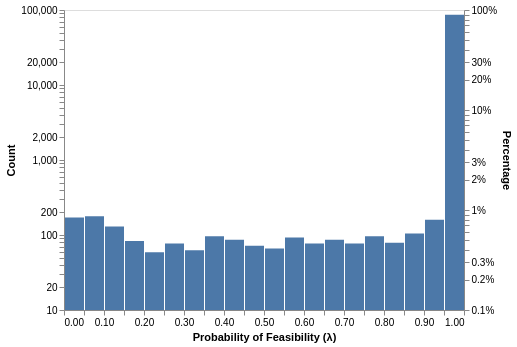
\includegraphics[width=\columnwidth]{irt_lambda_dist}
  \caption{
    The feasibility parameter $\lambda$ of our \irt{} model represents the probability that an example is unsolvable.
    For example, annotation error could lead to an example always being scored incorrectly---regardless of how good the model is.
    In \squad{} 2.0, $\lambda<.434$ in the $5\%$ percentile, $\lambda<.698$ for the $7.5\%$, and $\lambda<.931$ in the $10\%$ percentile.
  }
  \label{fig:lambda-dist}
\end{figure}

% \begin{figure*}[t]
%   \center
%   \tikz\node[draw=black!40!lightblue,inner sep=1pt,line width=0.3mm,rounded corners=0.1cm]{
%     \begin{tabular}{p{.95\textwidth}}
%       \textbf{Wikipedia Page}: \underline{Packet switching} \textbf{Question ID:} 5a551230134fea001a0e18d0 \\
%       \textbf{Question}: Late published versions were utilized by who?                                     \\
%       \textbf{Official Answer}: Not Answerable                                                             \\
%       \textbf{Plausible Answer}: \answer{Linux}                                                            \\
%       \textbf{Context}:
%       DECnet is a suite of network protocols created by Digital Equipment Corporation, originally released in 1975 in order to connect two PDP-11 minicomputers. It evolved into one of the first peer-to-peer network architectures, thus transforming DEC into a networking powerhouse in the 1980s. Initially built with three layers, it later (1982) evolved into a seven-layer OSI-compliant networking protocol. The DECnet protocols were designed entirely by Digital Equipment Corporation. However, DECnet Phase II (and later) were open standards with published specifications, and several implementations were developed outside DEC, including one for \answer{Linux}.
%     \end{tabular}
%   };

%   \caption{
%     TODO
%   }
%   \label{fig:ex-diff-easy}
% \end{figure*}



\section{Logistic Regression Features}
\label{ch:isicle:apx:features}

The linear model (\S\ref{ch:isicle:irt-accurate}) includes features based on \itm{} \abr{id}s, \subj{} \abr{id}s, textual features of the question, context, and answer, and topic model features.
Table~\ref{tab:vw-features} lists the feature names from Figure~\ref{fig:vw-ablation} with descriptions of each.
When \irt{} features or the statistics features are used, they include interaction terms with themselves.

\begin{table}[t]
  \centering
  \small
  % The table from here below is generated by code printed to terminal from:
  % leaderboard plot --plot irt_correlation
  \begin{tabular}{lp{.6\linewidth}}
    \toprule
    Feature                  & Description                                                                                                    \\
    \midrule
    All                      & All the features                                                                                               \\
    \irt{}                   & \irt{} values for \diff{}, \discability{}, feasibility, and ability                                            \\
    Item \abr{id}            & The item's \abr{id}                                                                                            \\
    Subject \abr{id}         & The subject's \abr{id}                                                                                         \\
    Question                 & Question words                                                                                                 \\
    Context                  & Context words                                                                                                  \\
    Stats                    & Question \& context lengths; answerability, answer position \& length; difficulty from~\citet{Sugawara2017-bm} \\
    Subject \& Item \abr{id} & Item and Subject \abr{id}                                                                                      \\
    Topics 1K                & Topic weights of question words                                                                                \\
    Title                    & Wikipedia page title words                                                                                     \\
    Baseline                 & No features, majority class baseline                                                                           \\
    \bottomrule
  \end{tabular}
  \caption{
    The linear model integrates a variety of features to determine which are most predictive of a \subj{} responding correctly to an \itm{}.
  }
  \label{tab:vw-features}
\end{table}

\section{IRT Model Type Correlation}
\label{apx:irt-self-corr}

Although each \irt{} model differs in expressiveness, they should---in general---produce similar results.
This is confirmed by computing the Kendall's rank correlation between the \subj{} abilities and \itm{} difficulties (Table~\ref{tab:irt-subj-corr}).

\begin{table}[t]
  \centering
  \small
  % The table from here below is generated by code printed to terminal from:
  % leaderboard plot --plot irt_correlation
  \begin{tabular}{lrrr}
    \toprule
    Ability & \pl{3}  & \pl{2}  & \pl{1}  \\
    \midrule
    \pl{3}  & $1.00$  & $0.947$ & $0.895$ \\
    \pl{2}  & $0.947$ & $1.00$  & $0.907$ \\
    \pl{1}  & $0.895$ & $0.907$ & $1.00$  \\
    \bottomrule
  \end{tabular}
  \caption{
    Table entries are Kendall's $\tau$ rank correlation of \irt{} \subj{} ability between rows and columns.
    Generally, the models agree on the ranking with the \pl{3}~and \pl{2}~having the strongest correlation.
  }
  \label{tab:irt-subj-corr}
\end{table}
\section{Ranking Stability Experiments}
\label{ch:isicle:apx:rank-stability}

Here we provide further details for the ranking stability experiments (\S\ref{ch:isicle:irt-compare}).
First, we filter from the $161$ \subjs{} that have development set scores to the $115$ that also have test set scores.\footnote{
  The \squad{} organizers curate the test set \subjs{} to avoid overfit, garbage, or duplicate submissions.
}
In our simulation, we run $10$ trials for every sample size; sample size begins at $100$ and with steps of $100$.
In addition to these, we also run trials for sample sizes 25, 50, and 75.
Since each sample can be no larger than half the dataset, we stop at half the dataset.

\subsection{Development and Test Set Correlations}
\begin{table}[t]
  \centering
  \small
  % The table from here below is generated by code printed to terminal from:
  % leaderboard plot --plot rank_correlation
  \begin{tabular}{lrrrr}
    \toprule
    {}                      & EM$_{\text{dev}}$ & EM$_{\text{test}}$ & Ability$_{\text{dev}}$ & Ability$_{\text{test}}$ \\
    \midrule
    EM$_{\text{dev}}$       & $1.00$            & $0.953$            & $0.954$                & $0.931$                 \\
    EM$_{\text{test}}$      & $0.953$           & $1.00$             & $0.944$                & $0.947$                 \\
    Ability$_{\text{dev}}$  & $0.954$           & $0.944$            & $1.00$                 & $0.950$                 \\
    Ability$_{\text{test}}$ & $0.931$           & $0.947$            & $0.950$                & $1.00$                  \\
    \bottomrule
  \end{tabular}
  \caption{
    Entries are Kendall's rank correlation between rows and columns.
    Scores are \squad{} Exact Match (EM) and \pl{2}~ability.
  }
  \label{tab:rank-corr}
\end{table}

Table \ref{tab:rank-corr} uses a \pl{2}~model since we noticed that in comparison~\pl{3}~overfit the data, yielding worse results.
The correlations with the full data are all strong, but not the same.
We conclude that---at least on \squad{}---\irt{} rankings are modestly more reliable than classical rankings.

\subsection{Statistical Significance of Difference in Kendall Tau Coefficients}
While Figure~\ref{fig:stability} shows a consistent difference in correlation between ranking methods, it is unclear whether this difference is statistically significant.
We estimate the statistical significance of the difference through bootstrap sampling~\citep{efron1994bootstrap}.

Since the null case is no difference in correlation coefficients, we seek a symmetric sampling distribution centered at zero that represents a realistic density function.
Each ranking stability experiment\footnote{One experiment for development sample to development sample and one for development sample to test set.} trial results in two lists of number pairs.
The lists correspond to \subj{} scores on two datasets;\footnote{
  In the first experiment, development set samples; in the second, a development set sample and the full test set.
} each number pair is the \subj{}'s accuracy and \irt{} score.
To create the bootstrap distribution, we (1) sample with replacement pairs from one list, (2) compute the correlation between the resampled ranking and unused ranking when using accuracy versus \irt{} score, and (3) compute and store the \irt{} correlation score minus the accuracy correlation score.
We repeat this process 1000 times for each of the 10 trials in the original experiment and aggregate all the differences to build the bootstrap distribution.
For each sample size we compute the empirical P-Value on each trial which we show in box and whisker plots (Figure~\ref{fig:rank_sig}).

\begin{figure*}[t]
  \centering
  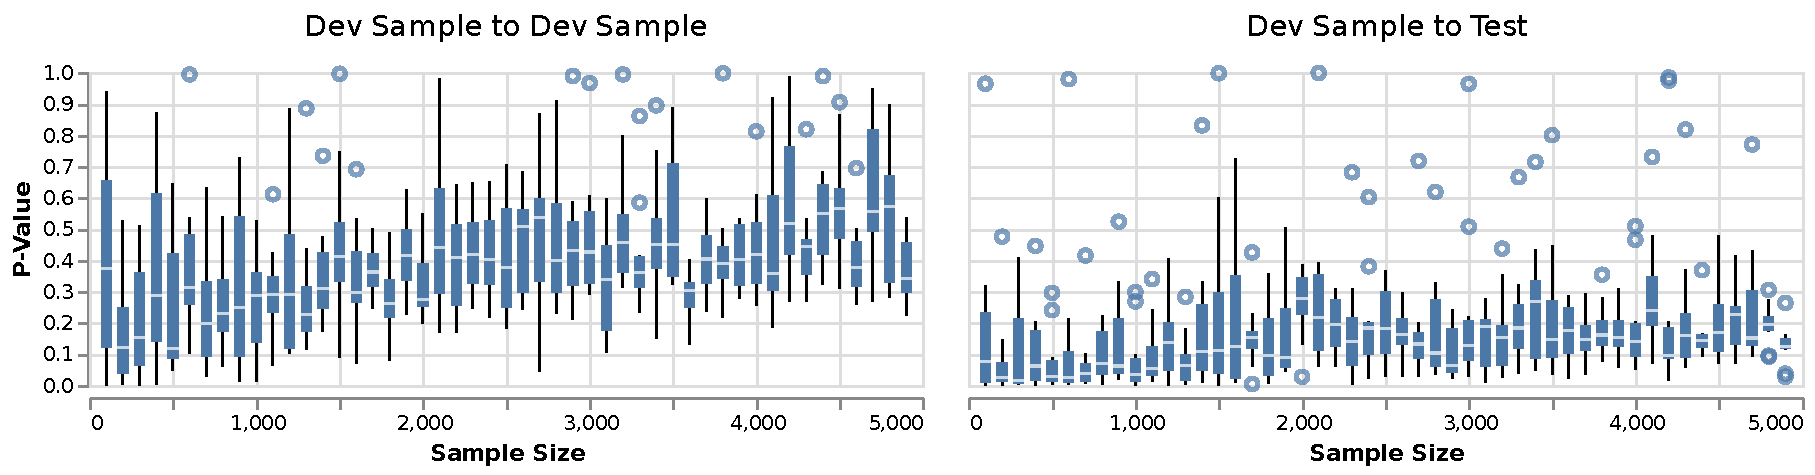
\includegraphics[width=\textwidth]{ranking_stability_significance}
  \caption{
    P-values of the rank correlation difference for each sample size and trial in Figure~\ref{fig:stability}.
    The inherent noise in dev set sampling makes inferring significance difficult (left); test set driven results (right) are more significant.
  }
  \label{fig:rank_sig}
\end{figure*}


\section{The IRT Statistical Test}
\label{ch:isicle:irt-test}

The \irt{} test differs in two substantial ways from other tests: (1) it does not assume that \itms{} are equally informative and (2) it does assume that the informativeness of \itms{} is a function of the \subj{}'s skill $\theta_j$.
In the literature, this is closely connected to \iemph{reliability}~\citep{sutcliffe1992pragmatics} and each \itm{} provides information about the location of $\theta_j$; as we accumulate more evidence for the location of $\theta_j$ the error of estimation decreases.
It is a well known result in \irt{} that standard error of estimate (\abr{see}) $\sigma(\hat{\theta}|\theta)$ varies with respect to the agent location parameter $\theta$~\citep[p.~30]{theory2013ayala} and is connected to the Fisher information
\begin{equation}
  I_i(\theta)=\frac{(p_i')^2}{p_i(1-p_i)}
\end{equation}
of each item.
For a 2PL model, information
\begin{equation}
  I_i(\theta)=\gamma^2p_i(1-p_i)
\end{equation}
is maximized when $p_i=(1-p_i)$.
Since Fisher information is additive, the information of the evaluation set is maximal when \itms{} have a $50\%$ chance of being responded to correctly.
As derived by~\citet[p.~102]{theory2013ayala}, the standard error of estimation
\begin{equation}
  \text{SEE}(\theta)=\sqrt{\frac{1}{\sum_i I_i(\theta)}}.
\end{equation}
is computed by accumulating the information gained from each \itm{}.
Given two \subjs{} $X$ and $Y$, one can use the probability distribution of score differences
\begin{equation}
  N(\theta_Y-\theta_X, \text{SEE}(\theta_X)^2+\text{SEE}(\theta_Y)^2)
\end{equation}
to compute the probability that the difference in skill is greater than two standard errors which corresponds to an $\alpha\le .05$ significance level.
%derive error apx~\citep{hambleton1991fundamentals}

\section{Multidimensional IRT Clustering}
\label{ch:isicle:clustering}

While we achieve strong held-out accuracy with 10 dimensional \irt{} (\pl{m}), we had limited success in interpreting parameters.
We use \abr{tsne}\footnote{
  We use openTSNE~\citep{policar2019tsne} with default parameters.
} plots overlayed with features like \itm{} accuracy, the question's Wikipedia page, if the question was answerable, length of questions, and topic model weights.
Of these, \itm{} accuracy and answerability showed the most obvious patterns (Figure~\ref{fig:tsne-squad}).

\begin{figure}[t]
  \centering
  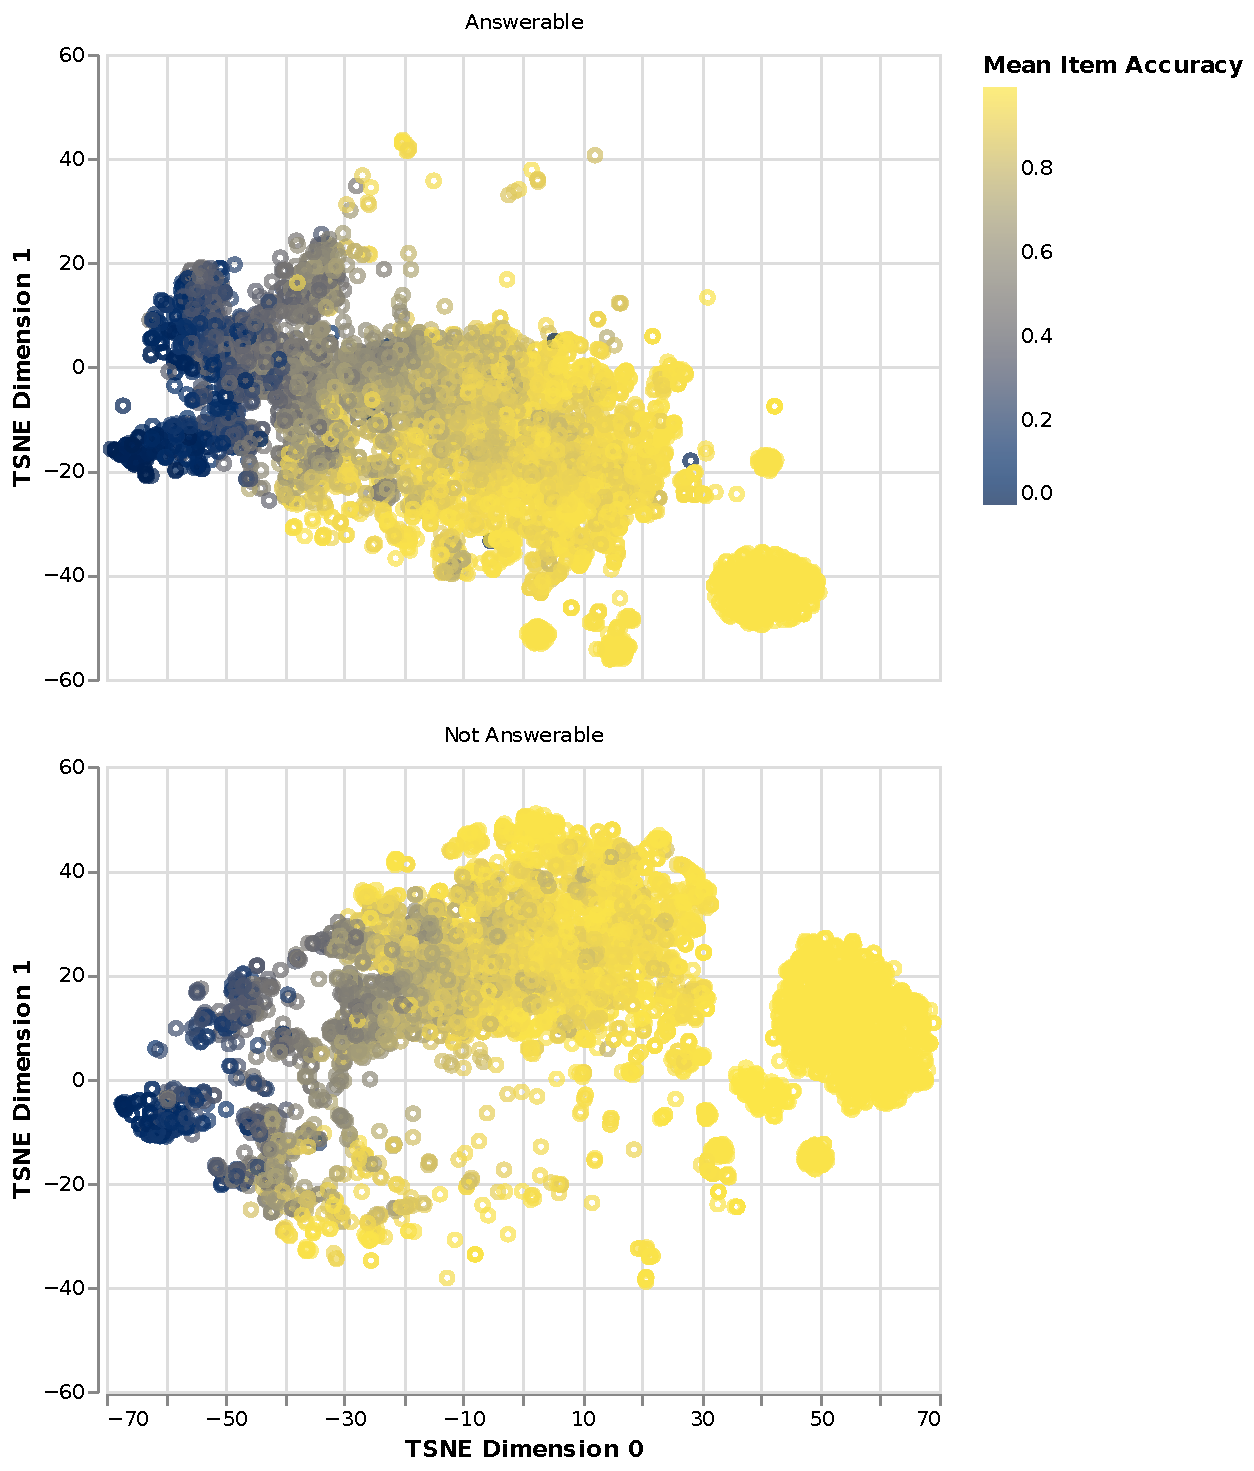
\includegraphics[width=\columnwidth]{squad_tsne}
  \caption{
    In \squad{}, \abr{tsne} shows a relationship between mean exact match (\itm{} accuracy) and answerability with respect to multidimensional \diff{} and \discability{}.
  }
  \label{fig:tsne-squad}
\end{figure}

We repeated this approach with the multi-task question answering shared task \abr{mrqa}~\citep{fisch2019mrqa}.
However, instead of using 10 dimensions we use 6 to match the number of development set tasks in \abr{mrqa}.
Although questions in NarrativeQA standout (Figure~\ref{fig:tsne-mrqa}), there is not a discernible pattern amongst the other tasks.
We leave more sophisticated methods for making multidimensional \irt{} models interpretable to future work.

\begin{figure}[t]
  \centering
  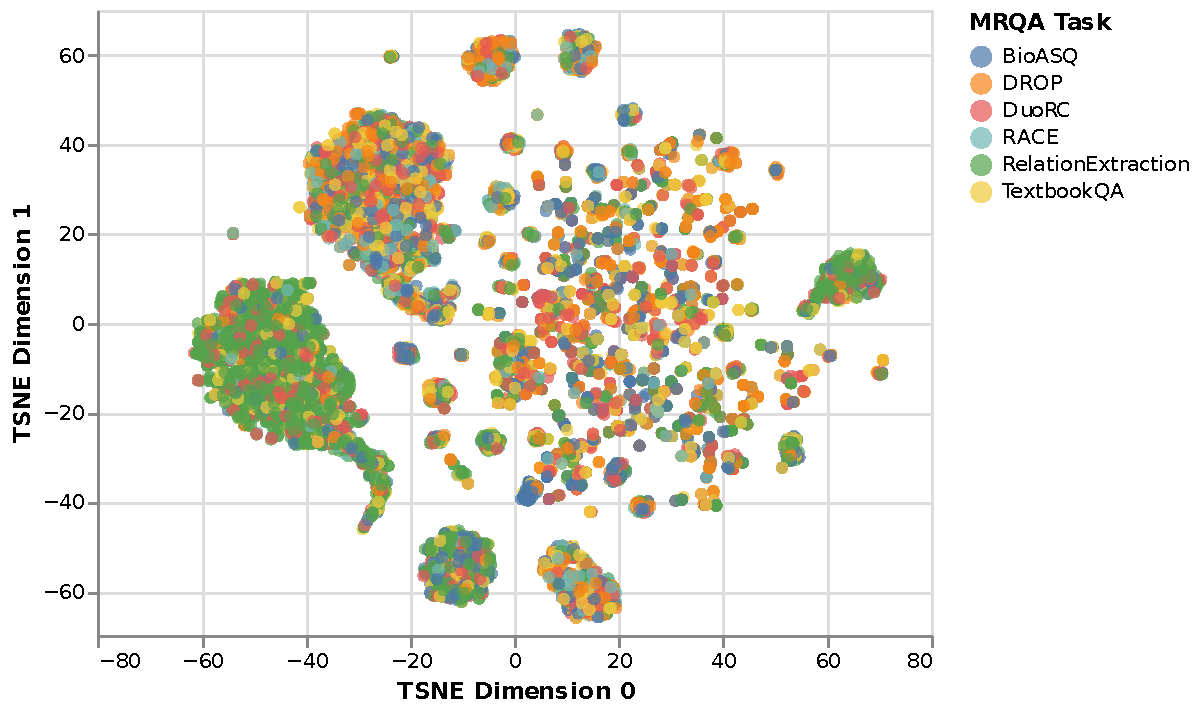
\includegraphics[width=\columnwidth]{mrqa_tsne}
  \caption{
    In \abr{mrqa}, \abr{tsne} shows a relationship between whether the task is NarrativeQA with respect to multidimensional \diff{} and \discability{}.
  }
  \label{fig:tsne-mrqa}
\end{figure}



\section{Reproducibility Checklist}

Here we provide reproducibility details to complement our source code (\href{https://irt.pedro.ai}{https://irt.pedro.ai}).

\subsection{Software and Parameters}

All \irt{} models are implemented in PyTorch~\citep{pytorch2019} and Pyro~\citep{bingham2018pyro}.
Linear models are trained with Vowpal Wabbit~\citep{Agarwal2014ARE}.
The topic model that generates features for the linear model uses Mallet~\citep{McCallumMALLET}.

The number of \irt{} model parameters is proportional to the number of \subjs{} $m$ and the number of \itms{} $n$.
The \pl{1}~has one parameter per \subj{} and one per \itm{}.
The \pl{2}~has one parameter per \subj{} and two per \itm{}.
The \pl{3}~has one parameter per \subj{} and three per \itm{}.
The \pl{m}~has ten parameters per \subj{} and thirty per \itm{}.

\subsection{Hyperparameters}

We did not invest significant effort in hyper-parameter tuning the \irt{} models and instead used the defaults in the py-irt software\footnote{\href{https://github.com/jplalor/py-irt}{github.com/jplalor/py-irt}} provided by~\citet{lalor2019latent}.
The \pl{1}, \pl{2}, and \pl{3}~models were trained for 1000 epochs with no early stopping conditions and a learning rate of $0.1$ with \abr{adam}~\citep{Kingma2014AdamAM}.
The \pl{m}~model was trained for 2500 epochs and used 10 dimensions.

In the linear model, we used a Hyperopt-based~\citep{bergstra2013hyperopt} tool provided by Vowpal Wabbit\footnote{
  \href{https://github.com/VowpalWabbit/vowpal_wabbit}{github.com/VowpalWabbit/vowpal\_wabbit}
} for hyper parameter search.
For each \abr{lm}, the tool spent 20 iterations optimizing the learning rate, L2 regularization, and number of bits against the logistic loss function.
The learning rate was searched from 0.001 to 10 with loguniform sampling, L2 regularization from $1e-8$ to 1, and bits from 20 to 23 as categorical variables.

The topic model that generated features for the linear model used mallet, and we followed the recommendations of the software to set hyper parameters.\footnote{
  \href{http://mallet.cs.umass.edu/topics.php}{mallet.cs.umass.edu/topics.php}
}
Specifically, we used an optimization interval of 10, removed stop words, trained for 1000 iterations, and used a document-topic threshold of 0.05.
Each document was comprised of the Wikipedia page title and the question text.

\subsection{Computational Resources}

The majority of experiments were conducted on a single workstation with an Intel i7-7700K \abr{cpu}, $47$\abr{gb} of \abr{ram}, and an Nvidia 1080Ti.
The average runtime for the \pl{3}~model on \abr{cpu} is 113 seconds with a standard deviation of 2.31 over 5 trials.
The average runtime of the \pl{m}~model on \abr{gpu} is 110 seconds with a standard deviation of 0.5 over 5 trials.

Since each ranking stability experiment required (\S\ref{ch:isicle:stable}) re-training an \pl{3}~model on each subset, we parallelized this experiment on a \abr{cpu} cluster where each trial received two \abr{cpu} cores and 16\abr{gb} of \abr{ram}.
In total, this included 520 trials which corresponds to twice that many trained \irt{} models since one model is trained on each subset of the data.

\end{appendix}
\end{document}
